\documentclass[runningheads,11pt]{llncs}

\usepackage[T1]{fontenc}
\usepackage{lmodern}
\usepackage{amsmath,amssymb}
\usepackage{alltt}
\usepackage{booktabs}
\usepackage{array}
\usepackage{tikz}
\usetikzlibrary{arrows.meta,positioning,calc,fit,shapes.misc}
\usepackage{algorithm}
\usepackage[noend]{algpseudocode}
\usepackage[hidelinks]{hyperref}

\DeclareUrlCommand\lean{\urlstyle{tt}}
\DeclareUrlCommand\file{\urlstyle{tt}}
\newcommand{\efxz}{\texorpdfstring{\mbox{EFX$_0$}}{EFX0}}
\newcommand{\LBp}{\texorpdfstring{\mbox{LB$^{+}$}}{LB+}}
\newcommand{\NA}{\mathit{NA}}
\newcommand{\capa}{\mathrm{cap}}
\newcommand{\base}{\mathrm{base}}
\newcommand{\none}{\bot}
\newcommand{\st}{\mathrel{:}}
\newcommand{\HitSet}{\textup{\textsc{HitSet}}}
\newcommand{\Complete}{\textup{\textsc{Complete}}}
\algrenewcommand\algorithmiccomment[1]{\hfill$\triangleright$ #1}

\begin{document}

\title{\efxz{} Allocations with at Most Three Relevant Goods: Existence and a Verified Polynomial-Time Algorithm}
\subtitle{Long version}
\titlerunning{\efxz{} with at Most Three Relevant Goods (long version)}

\author{Evan Lin}
\authorrunning{E. Lin}
\institute{University of Illinois Urbana-Champaign}

\maketitle

\begin{abstract}
An allocation of indivisible goods is \efxz{} if no agent envies another agent's bundle after removing any single good from it, even a good that the envious agent values at zero. We prove that every instance with nonnegative additive valuations in which each agent positively values at most three goods has a complete \efxz{} allocation, and we give a polynomial-time algorithm, K3ALG, that computes one. K3ALG first lets agents leave with a good they value at least as much as all their other remaining goods together. The remaining agents pick goods in a serial dictatorship that serves agents who have lost a good first; the leftover goods fill free slots, and the surplus goes to a single owner, after at most one rotation of picks along a chain of agents. For natural-number values, the correctness of K3ALG and a polynomial bound on its number of operations are machine-checked in Lean~4 on the program itself; the existence results are machine-checked over any linearly ordered cancellative commutative monoid, such as the nonnegative reals. If every agent values exactly three goods, none more than the other two together, some \efxz{} allocation gives more than two goods to at most one agent. This long version is meant to be read on its own: it explains the approach informally, traces the algorithm on two examples, and gives every proof of the main theorems in full.
\keywords{Fair division \and Indivisible goods \and EFX \and Serial dictatorship \and Formal verification \and Lean}
\end{abstract}

\section{Introduction}\label{sec:intro}

\subsection{EFX and \efxz{}}\label{sec:intro-efx}

We allocate a set $M$ of $m$ indivisible goods to a set $N$ of $n$ agents. Agent $i$ has an \emph{additive valuation}: a value $v_i(g)\ge0$ for each good $g$, and $v_i(S)=\sum_{g\in S}v_i(g)$ for every set $S$ of goods. An \emph{allocation} $X=(X_i)_{i\in N}$ gives agent $i$ the \emph{bundle} $X_i$; bundles are pairwise disjoint, and the allocation is \emph{complete} if they cover $M$. Every allocation in this paper is complete: no good may be thrown away.

Envy-freeness, $v_i(X_i)\ge v_i(X_j)$ for all agents $i$ and $j$, can be impossible with indivisible goods; think of one good and two agents who both value it. \emph{Envy-freeness up to any good} weakens it~\cite{AmanatidisBFV22}: agent $i$ may envy the bundle $X_j$, but the envy must disappear as soon as any single good is removed from $X_j$. Two versions of this idea are in use. They differ in which goods may be removed:
\begin{align*}
\text{EFX:}&\quad v_i(X_i)\ge v_i(X_j\setminus\{h\})\quad\text{for all } i\ne j \text{ and } h\in X_j \text{ with } v_i(h)>0;\\
\text{\efxz{}:}&\quad v_i(X_i)\ge v_i(X_j\setminus\{h\})\quad\text{for all } i\ne j \text{ and } h\in X_j.
\end{align*}
Both conditions are vacuous when $X_j$ is empty. \efxz{} implies EFX, and the two coincide when all values are positive. Whether every instance with additive valuations has a complete EFX allocation is a central open question of fair division~\cite{AmanatidisBFV22}. Most known existence results (Section~\ref{sec:related}) are proved in the stronger form \efxz{}.

The two notions differ exactly on goods that the envious agent values at zero, and such goods are what this paper is about.

\begin{example}[EFX, but not \efxz{}]\label{ex:efx-vs-efx0}
Two agents share three goods $a$, $b$, $c$. Agent~1 values $a$ at $3$, $b$ at $2$ and $c$ at $0$; agent~2 values only $c$, at $1$. Consider $X_1=\{b\}$ and $X_2=\{a,c\}$. Under EFX, agent~1 may remove only $a$ from $X_2$, since $c$ is worthless to it; what remains, $\{c\}$, is worth $0\le2$. Agent~2 holds $c$ and faces the single good $b$, which it values at $0$. So $X$ is EFX. It is not \efxz{}: removing $c$ from $X_2$ leaves $\{a\}$, worth $3>2$ to agent~1. The allocation $X_1=\{a\}$, $X_2=\{b,c\}$ is \efxz{}.
\end{example}

The example shows a general mechanism. If $X_j$ contains a good $h$ that agent $i$ values at zero, then $v_i(X_j\setminus\{h\})=v_i(X_j)$, so \efxz{} requires $v_i(X_i)\ge v_i(X_j)$: agent $i$ must not envy $X_j$ at all. When every agent values only a few goods, most bundles contain goods that a given agent values at zero, and \efxz{} is close to plain envy-freeness towards every bundle of two or more goods. Two consequences run through the whole paper:
\begin{itemize}
\item a good that nobody values cannot simply be handed to an arbitrary agent, because it turns every constraint towards that agent's bundle into envy-freeness; and
\item a good that agent $j$ values but agent $i$ does not cannot join a bundle that $i$ envies.
\end{itemize}

\subsection{The question and the answer}\label{sec:answer}

Write $R_i=\{g\in M\st v_i(g)>0\}$ for the goods agent $i$ values, its \emph{relevant} goods. An instance is \emph{$k$-relevant} if $|R_i|\le k$ for every agent $i$. For $k\le2$, serial dictatorship works: the agents, in any order, each take a favourite remaining good, and the last agent takes everything left. The result is \efxz{} (this is machine-checked in~\cite{MrdEfx}; we reprove it as Corollary~\ref{cor:k2}). At $k=3$ serial dictatorship breaks. An agent that values $a$, $b$, $c$ at $4$, $3$, $2$ may take $a$ and then see $b$ and $c$ end up in the last agent's bundle together with a third good; removing that third good, which it values at zero, leaves $b$ and $c$, worth $5>4$.

This paper answers the question for $k=3$.

\begin{theorem}[existence]\label{thm:target}
Every instance with $n\ge1$ agents and nonnegative real additive valuations in which every agent positively values at most three goods has a complete \efxz{} allocation.
\end{theorem}

\noindent Call an agent that values exactly three goods, ranked $a\succ b\succ c$ by value, \emph{balanced} if it values $a$ at most as much as $b$ and $c$ together.

\begin{theorem}[one large bundle]\label{thm:D}
Every instance with $n\ge1$ agents and nonnegative real additive valuations in which every agent values exactly three goods and is balanced has a complete \efxz{} allocation in which every agent except at most one receives at most two goods.
\end{theorem}

\noindent The third result is an algorithm. We measure its running time in the \emph{unit-cost model}, where each list step, comparison of agents or goods, read of an input value or table entry, and comparison or addition of natural numbers of any size costs one operation (Section~\ref{sec:time} states the model precisely, and Corollary~\ref{cor:bits} removes the assumption that numbers of any size cost one unit).

\begin{theorem}[algorithm]\label{thm:algo}
Given $n\ge1$ agents, $m$ goods and natural-number values in binary, algorithm K3ALG (Section~\ref{sec:algo}) performs at most $400(n+m+1)^4$ operations in the unit-cost model. If every agent positively values at most three goods, it returns a complete \efxz{} allocation.
\end{theorem}

\begin{corollary}[rational values; written, not formalized]\label{cor:rat}
By scaling each agent's values to integers, which preserves every comparison between sums of that agent's values, K3ALG applies to nonnegative rational valuations.
\end{corollary}

\noindent The proofs of Theorems~\ref{thm:target}--\ref{thm:algo} are written in full in this paper and are also machine-checked in Lean~4 (Section~\ref{sec:lean}). Table~\ref{tab:status} lists every claim of the paper with its status; the corollaries marked ``written, not formalized'' have complete written proofs but are not machine-checked.

\begin{table}[tbp]
\caption{The claims of this paper. \emph{In Lean}: machine-checked (Section~\ref{sec:lean}); $^*$over any linearly ordered cancellative commutative monoid, such as $\mathbb{R}_{\ge0}$ (the Lean library has no real numbers, and that $\mathbb{R}_{\ge0}$ is such a monoid is the textbook fact used). \emph{Proved}: a complete written proof in this paper. \emph{Computation}: exhaustive, with independently re-checked certificates. \emph{Measured}: evidence only.}\label{tab:status}
\centering\small
\setlength{\tabcolsep}{4pt}\begin{tabular}{@{}llll@{}}
\toprule
Claim & Values & In Lean? & Status \\
\midrule
Thm.~\ref{thm:target}: existence & $\mathbb{R}_{\ge0}$ & yes$^*$ & proved \\
Thm.~\ref{thm:D}: one large bundle & $\mathbb{R}_{\ge0}$ & yes$^*$ & proved \\
Thm.~\ref{thm:algo}: K3ALG is correct & $\mathbb{N}$ & yes & proved \\
Thm.~\ref{thm:algo}: $400(n+m+1)^4$ operations (unit cost) & $\mathbb{N}$ & yes & proved \\
Prop.~\ref{prop:size}: size of the large bundle & $\mathbb{R}_{\ge0}$ & no & proved \\
Cor.~\ref{cor:bits}: bit complexity & $\mathbb{N}$ & no & proved \\
Cor.~\ref{cor:rat}: rational values & $\mathbb{Q}_{\ge0}$ & no & proved \\
Cor.~\ref{cor:real}: real values, comparison oracle & $\mathbb{R}_{\ge0}$ & no & proved \\
Sect.~\ref{sec:finer}: $O(n^4+n^2m)$ operations & $\mathbb{N}$ & no & written analysis \\
Sect.~\ref{sec:cert}: existence for $n\le7$ & $\mathbb{R}_{\ge0}$ & no & computation \\
Sect.~\ref{sec:finer}: speed of an implementation & $\mathbb{N}$ & no & measured \\
\bottomrule
\end{tabular}
\end{table}

\paragraph{Why this is not a corollary of known results.} A $3$-relevant instance without a complete \efxz{} allocation would refute the additive EFX conjecture itself. Indeed, adding a small $\varepsilon>0$ to every value gives an instance with positive values, in which EFX and \efxz{} coincide. If each of these perturbed instances had an EFX allocation, one allocation would serve arbitrarily small $\varepsilon$, since there are finitely many allocations, and it would be \efxz{} for the original values, since the inequalities are closed (compare~\cite[Lemma~1]{ChaudhuryGM20}). But the perturbation makes every good relevant to every agent, so it destroys the structure we exploit, and no published result that we know of implies Theorem~\ref{thm:target}~\cite{Repo}. Theorem~\ref{thm:target} gives one, with a machine-checked polynomial-time algorithm.

\subsection{Related work}\label{sec:related}

For additive valuations, complete EFX allocations are known to exist only in special cases, several of them in recent preprints: for three agents~\cite{ChaudhuryGM20}; when $m\le n+3$~\cite{Mahara21}; for four agents and at most nine goods~\cite{AlkassarFM26}; when every good is valued by at most two agents (graphs and multigraphs of agents, with goods as edges)~\cite{AfshinmehrAMMS26,ChristodoulouFKS23,SgouritsaS25,KavianiSS24}; and for hypergraphs of girth at least four~\cite{LianeasSS26}. All of these use the all-goods form \efxz{}; the graph results allow goods of value zero to the agents they are incident to, and for results that bound $n$ and $m$ positive values suffice by the perturbation argument above. For monotone valuations that are not additive, EFX allocations need not exist~\cite{AkramiMMSW26,MackenzieS26}.

We restrict instead how many goods each agent values. For $k\le2$, serial dictatorship suffices and has been formalized in Lean~\cite{MrdEfx}. For $k\le4$, Viswanathan and Mehta~\cite{ViswanathanM24} announce the existence of ordinary EFX allocations, with a polynomial-time algorithm and a proof sketch in an extended abstract. Their first phase, which serves agents whose top good outweighs their other two goods, resembles our rule R1 (Section~\ref{sec:peel}). Their algorithm ends by giving the goods that nobody values to an arbitrary agent, which is harmless for EFX but can break \efxz{}, as Example~\ref{ex:efx-vs-efx0} illustrates. Goods that nobody values are in fact easy to place (Lemma~\ref{lem:junk}); the difficulty under \efxz{} comes from goods that one agent values and another does not, which their EFX argument does not need to address. Since \efxz{} implies EFX, Theorem~\ref{thm:target} proves the case $k=3$ of their result in full.

\subsection{How to read this paper}\label{sec:roadmap}

Section~\ref{sec:overview} explains the approach in plain words on one instance, with no formal definitions. Section~\ref{sec:prelim} gives the model and four basic lemmas: the ordinal description of when an agent is safe (Lemma~\ref{lem:L5}), on which the whole design rests; peeling; goods valued by nobody; and the reduction of real values to natural numbers. Section~\ref{sec:algo} defines the algorithm K3ALG one notion at a time, lists it as pseudocode, and traces it on two examples, one with an owner and one with a rotation. Section~\ref{sec:correct} proves it correct, with every case written out. Section~\ref{sec:time} bounds its running time. Section~\ref{sec:lean} describes the Lean formalization: what it covers, what must be trusted, and how to read its statements. Section~\ref{sec:cert} reports the exhaustive computations for small instances and shows, by counterexamples, that the shape of Theorem~\ref{thm:D} cannot be improved in the obvious ways. Section~\ref{sec:concl} concludes.

The paper is self-contained. Its claims are also recorded, each with its evidence, in the ledger of the public repository~\cite{Repo}. Every example in this paper was checked by running the repository's implementation of K3ALG together with a brute-force check of the \efxz{} definition; the two main examples were also evaluated by the Lean program itself (Appendix~\ref{app:examples}).

\section{Overview of the Approach}\label{sec:overview}

This section explains the algorithm in plain words, on one instance, before any formal definition. Figure~\ref{fig:pipeline} shows its stages. Section~\ref{sec:algo} gives the precise definitions and traces the same instance step by step (Example~\ref{ex:owner}); Section~\ref{sec:correct} proves everything claimed here.

\begin{figure}[tbp]
\centering
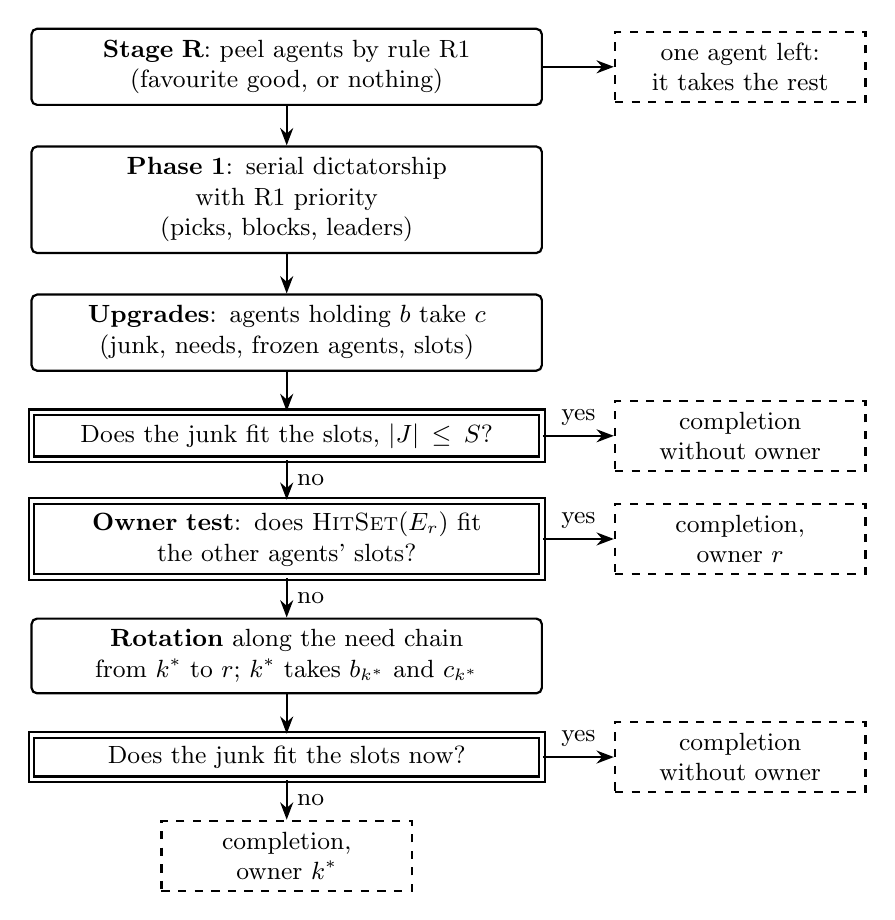
\begin{tikzpicture}[
  font=\small,
  box/.style={draw, thick, rounded corners=2pt, align=center, inner sep=4pt, text width=6.2cm},
  test/.style={draw, thick, align=center, inner sep=4pt, text width=6.2cm, double, double distance=1.2pt},
  outb/.style={draw, thick, dashed, align=center, inner sep=4pt, text width=2.9cm},
  arr/.style={-{Stealth[length=2.2mm]}, thick},
  node distance=5mm]
\node[box] (R) {\textbf{Stage R}: peel agents by rule R1\\(favourite good, or nothing)};
\node[box, below=of R] (P) {\textbf{Phase 1}: serial dictatorship\\with R1 priority\\(picks, blocks, leaders)};
\node[box, below=of P] (U) {\textbf{Upgrades}: agents holding $b$ take $c$\\(junk, needs, frozen agents, slots)};
\node[test, below=of U] (T1) {Does the junk fit the slots, $|J|\le S$?};
\node[test, below=of T1] (T2) {\textbf{Owner test}: does $\HitSet(E_r)$ fit\\the other agents' slots?};
\node[box, below=of T2] (Rot) {\textbf{Rotation} along the need chain\\from $k^*$ to $r$; $k^*$ takes $b_{k^*}$ and $c_{k^*}$};
\node[test, below=of Rot] (T3) {Does the junk fit the slots now?};
\node[outb, below=of T3] (O4) {completion,\\owner $k^*$};
\node[outb, right=9mm of T1] (O1) {completion\\without owner};
\node[outb, right=9mm of T2] (O2) {completion,\\owner $r$};
\node[outb, right=9mm of T3] (O3) {completion\\without owner};
\node[outb, right=9mm of R] (O0) {one agent left:\\it takes the rest};
\draw[arr] (R) -- (P); \draw[arr] (P) -- (U); \draw[arr] (U) -- (T1);
\draw[arr] (T1) -- node[right]{no} (T2); \draw[arr] (T2) -- node[right]{no} (Rot); \draw[arr] (Rot) -- (T3);
\draw[arr] (T3) -- node[right]{no} (O4);
\draw[arr] (T1) -- node[above]{yes} (O1); \draw[arr] (T2) -- node[above]{yes} (O2); \draw[arr] (T3) -- node[above]{yes} (O3);
\draw[arr] (R) -- (O0);
\end{tikzpicture}
\caption{The stages of K3ALG. Dashed boxes are outputs; double-bordered boxes are tests. Stage R ends when rule R1 applies to no agent (then Phase 1 starts) or when at most one agent or no good is left (then the algorithm returns). Every output is a completion of the current pre-allocation; the owner, if any, receives the only bundle that may have more than two goods.}\label{fig:pipeline}
\end{figure}

\paragraph{The instance.} Five agents share nine goods $g_0,\dots,g_8$. Each agent's positive values are, from the most to the least valued good:
\begin{center}
\setlength{\tabcolsep}{4pt}\begin{tabular}{@{}l@{\ \ }l@{\qquad}l@{\ \ }l@{}}
agent 0: & $g_2\mapsto6$, $g_4\mapsto5$, $g_6\mapsto2$ & agent 3: & $g_2\mapsto9$, $g_8\mapsto8$, $g_1\mapsto7$ \\
agent 1: & $g_6\mapsto5$, $g_7\mapsto4$, $g_0\mapsto3$ & agent 4: & $g_5\mapsto6$ \\
agent 2: & $g_2\mapsto9$, $g_1\mapsto7$, $g_3\mapsto5$ & & \\
\end{tabular}
\end{center}
Every other value is $0$. Note that $g_2$ is the favourite good of three agents.

\paragraph{Step 1: peeling.} Agent~$4$ values only $g_5$. If it takes $\{g_5\}$ and leaves, then whatever the others do afterwards, agent~4 values every other bundle at $0$, and nobody can strongly envy a bundle of one good: removing that good leaves nothing. More generally, an agent whose favourite remaining good $p$ is worth at least as much as all its other remaining goods together may take $\{p\}$ and leave (\emph{rule R1}, Lemma~\ref{lem:peel}); an agent that values none of the remaining goods may leave with nothing. We repeat this while it applies. In the example only agent~$4$ leaves: agent~$0$, for instance, values its favourite $g_2$ at $6<5+2$.

When peeling stops, every remaining agent values exactly three of the remaining goods, $a\succ b\succ c$, and is \emph{strictly balanced}: $v(a)<v(b)+v(c)$ (Lemma~\ref{lem:R1fail}). An agent valuing at most two goods, or with $v(a)\ge v(b)+v(c)$, would still be peeled.

\paragraph{Step 2: a serial dictatorship with R1 priority.} The remaining agents now take turns, and each takes its favourite good among those still available: its \emph{pick}. The order matters. If some waiting agent has already lost one of its goods, it goes next. Such an agent has at most two of its goods left, so rule R1 holds for it in the remaining instance, and taking its favourite good is safe for the same reason as peeling. Only when every waiting agent still has all three of its goods does a new agent, a \emph{leader}, take its top good $a$. A leader and the agents served after it, up to the next leader, form a \emph{block}.

In the example all four agents start with all their goods, so agent~$0$ (the first in index order) leads block~1 and picks $g_2$. Agents~$2$ and~$3$ have lost $g_2$: agent~$2$ picks its $b=g_1$, and then agent~$3$, which has lost $g_2$ and $g_1$, picks its $b=g_8$. The only agent still waiting, agent~$1$, has all its goods; it leads block~2 and picks its top, $g_6$. Four goods are left over: $g_0$, $g_3$, $g_4$, $g_7$.

\paragraph{Step 3: why the leftovers are the whole difficulty.} If no good were left over, every agent would hold at most one good, and the allocation would be \efxz{} for the trivial reason that nobody can strongly envy a bundle of at most one good. The leftovers, which we call \emph{junk}, must go somewhere, and in general they create bundles of two or more goods, which can be strongly envied. Lemma~\ref{lem:L5} says exactly when a strictly balanced agent with $v(a)>v(b)>v(c)$ is safe:
\begin{itemize}
\item holding $a$, it is safe unless $b$ and $c$ lie together in a bundle of three or more goods;
\item holding $b$ and $c$, it is always safe;
\item holding only $b$ of its goods, it is safe if and only if $a$ is \emph{alone} (the only good of its bundle);
\item holding only $c$, it is safe if and only if $a$ and $b$ are alone;
\item holding none of its goods, it is safe if and only if $a$, $b$ and $c$ are all alone.
\end{itemize}
So an agent that lost goods to earlier agents is safe as long as those goods stay alone. We call them its \emph{needs}. In the example, agent~$2$ holds its $b$ and needs $g_2$ alone, and agent~$3$ holds its $b$ and needs $g_2$ alone too. So $g_2$, agent~$0$'s pick, must stay alone: agent~$0$ may receive no junk. Such an agent is \emph{frozen}.

\paragraph{Step 4: slots and upgrades.} An agent whose pick nobody needs, a \emph{terminal}, may receive one junk good (a \emph{slot}), and an agent without a pick may receive two. An agent that picked its $b$ and whose $c$ is junk may also take its $c$ (an \emph{upgrade}): holding $b$ and $c$ is always safe, and the agent then needs nothing. The upgrade is allowed only if nobody needs its $b$ alone, since $b$ will now share a bundle. In the example, agent~$2$ holds $b=g_1$, its $c=g_3$ is junk, and nobody needs $g_1$, so agent~$2$ takes $g_3$. Agent~$3$ cannot upgrade: its $c=g_1$ belongs to agent~$2$. Now agent~$0$ is frozen (agent~$3$ still needs $g_2$), agents~$1$ and~$3$ are terminals with one slot each, and the junk is $g_0$, $g_4$, $g_7$: three goods for two slots.

\paragraph{Step 5: the owner.} When the junk exceeds the slots, one agent, the \emph{owner}, takes all the junk that does not fit, so its bundle has three or more goods. By Lemma~\ref{lem:L5}, such a bundle can hurt only an agent $x$ that holds its top $a_x$ and would find both $b_x$ and $c_x$ in it. Such an agent is \emph{exposed}, and it is protected if one of $b_x$, $c_x$ goes into a slot instead. The natural candidate owner is $r$, the last agent served that is not upgraded; here $r=1$. Agent~$0$ is exposed for $r$: it holds its top $g_2$, its $b=g_4$ is junk, and its $c=g_6$ is $r$'s own pick. So $g_4$ goes into agent~$3$'s slot and the owner takes $g_0$ and $g_7$:
\[
X_0=\{g_2\},\ X_1=\{g_6,g_0,g_7\},\ X_2=\{g_1,g_3\},\ X_3=\{g_8,g_4\},\ X_4=\{g_5\}.
\]
This allocation is \efxz{}; Table~\ref{tab:ex1check} checks it agent by agent. Filling agent~$3$'s slot with $g_0$ instead would give the owner $\{g_6,g_4,g_7\}$. Agent~$0$ values that bundle at $7>6$ and still at $7$ after removing $g_7$, which it values at zero, so the allocation would not be \efxz{}. It would still be EFX, since removing $g_4$ or $g_6$ leaves $2$ or $5$: here, again, the difference between the two notions is a good worthless to the envious agent.

Why does $r$ usually work? An exposed agent took its top while $b$ and $c$ were still available, so it found all three of its goods available: it is a leader. So different exposed agents lead different blocks. Each of them has a slot at its disposal inside its own block: its own, if it is a terminal; if it is frozen, the slot of the terminal at the end of a chain of needs inside the block (a \emph{need chain}). In the example, agent~$3$ needs agent~$0$'s pick and is a terminal, so the need chain is $0\to3$, and agent~$3$'s slot protects agent~$0$. So there is one slot per exposed agent, except possibly for the exposed agent in $r$'s own block, because $r$'s own slot is not available to others.

\paragraph{Step 6: the one rotation.} The count above fails in exactly one situation, the \emph{bad case} (Theorem~\ref{thm:A}): the leader $k^*$ of $r$'s block is exposed and frozen, every need chain from $k^*$ ends at $r$, and no two exposed agents can be protected by the same junk good. Then we rotate along the need chain from $k^*$ to $r$: every agent of the chain takes the good it needed from its predecessor, and $k^*$ gives up its top $a$ and takes $b$ and $c$ instead (an upgrade). Every agent of the chain now holds a good it ranks above its old pick, so the goods that must stay alone can only become fewer, and $k^*$ can now own the large bundle (Theorem~\ref{thm:B}). Example~\ref{ex:rot} in Section~\ref{sec:algo} shows a rotation, and Figure~\ref{fig:rot} draws it.

\paragraph{What is proved.} The allocation that K3ALG returns is \efxz{} whenever every agent values at most three goods (Theorem~\ref{thm:algo}), and at most one agent of Stage L, the owner, receives more than two goods. The proof in Section~\ref{sec:correct} works for every order of the dictatorship with R1 priority and every order of the upgrades, so K3ALG's choice of the smallest index is only one way to break ties.

\section{Preliminaries}\label{sec:prelim}

\subsection{Model and notation}\label{sec:model}

An \emph{instance} consists of a finite set $N$ of $n\ge1$ agents, a finite set $M$ of $m$ goods, and nonnegative additive valuations $v_i$, $i\in N$. Agents and goods are numbered, and ``index order'' and ``the first'' refer to these numbers; in examples, agents are $0,1,2,\dots$ and goods are $g_0,g_1,\dots$. The relevant goods of agent $i$ are $R_i=\{g\in M\st v_i(g)>0\}$. An allocation $X$ is \emph{\efxz{}} if every agent is \emph{safe} in it, where agent $i$ is safe in $X$ if
\[
  v_i(X_i)\ \ge\ v_i(X_j\setminus\{h\})\qquad\text{for every agent } j\ne i \text{ and every good } h\in X_j .
\]
It is convenient to name the largest right-hand side. For a nonempty set $B$ of goods, the \emph{threat} of $B$ to agent $i$ is
\[
  \theta_i(B)\;=\;\max_{h\in B} v_i(B\setminus\{h\})\;=\;v_i(B)-\min_{h\in B}v_i(h),
\]
and $\theta_i(\emptyset)=0$. Agent $i$ is safe in $X$ if and only if $v_i(X_i)\ge\theta_i(X_j)$ for every $j\ne i$. A good is \emph{alone} in $X$ if it is the only good of its bundle.

\begin{lemma}[threats]\label{lem:threat}
Let $B$ be a set of goods and $i$ an agent. (a) If $|B|\le1$, then $\theta_i(B)=0$: a bundle of at most one good is never strongly envied. (b) If $B$ contains a good outside $R_i$, then $\theta_i(B)=v_i(B)$. (c) In every case $\theta_i(B)\le v_i(B)$, and $\theta_i(B)$ depends only on the values $v_i(g)$, $g\in B$.
\end{lemma}

\begin{proof}
By additivity, $v_i(B\setminus\{h\})=v_i(B)-v_i(h)$ is largest when $v_i(h)$ is smallest. (a) If $B=\{h\}$, removing $h$ leaves nothing. (b) The smallest value in $B$ is then $0$. (c) Values are nonnegative. \qed
\end{proof}

\noindent Part (b) is the mechanism of Example~\ref{ex:efx-vs-efx0}: towards a bundle that contains a good it does not value, an agent needs full envy-freeness.

\subsection{Rankings and balance}\label{sec:balance}

When $|R_i|=3$ we name agent $i$'s relevant goods $a_i$, $b_i$, $c_i$ so that $v_i(a_i)\ge v_i(b_i)\ge v_i(c_i)>0$, breaking ties between equal values by index (the good with the smaller index comes first). This gives a strict \emph{ranking} $a_i\succ_i b_i\succ_i c_i$, fixed once and for all; we write $g\succ_i h$ when $i$ ranks $g$ above $h$. Agent $i$ is
\begin{itemize}
\item \emph{balanced} if $v_i(a_i)\le v_i(b_i)+v_i(c_i)$, that is, if no relevant good is worth more than the other two together (equivalently, $2v_i(g)\le v_i(M)$ for every good $g$, the form used in Lean);
\item \emph{strictly balanced} if $v_i(a_i)<v_i(b_i)+v_i(c_i)$;
\item \emph{top-heavy} if $v_i(a_i)\ge v_i(b_i)+v_i(c_i)$.
\end{itemize}
Much of the paper depends on the values only through the rankings. Given rankings $a_i\succ_i b_i\succ_i c_i$ of three goods per agent, a valuation is \emph{consistent} with them if $v_i(a_i)\ge v_i(b_i)\ge v_i(c_i)>0$ and $v_i(g)=0$ for every other good, for every agent $i$.

\subsection{When is an agent safe? The ordinal lemma}\label{sec:L5}

The next lemma describes exactly when a strictly balanced agent with three relevant goods is safe. It is the key to the design of the algorithm: every notion of Section~\ref{sec:algo} comes from one of its cases.

\begin{lemma}[cases of safety]\label{lem:L5}
Let agent $i$ have $R_i=\{a,b,c\}$ with $v_i(a)>v_i(b)>v_i(c)>0$ and $v_i(a)<v_i(b)+v_i(c)$, and let $X$ be an allocation.
\begin{enumerate}
\item[(i)] The eight sums of subsets of $\{a,b,c\}$ are ordered as $0<c<b<a<b+c<a+c<a+b<a+b+c$, writing $x$ for $v_i(x)$.
\item[(ii)] Agent $i$ is safe in $X$ if and only if one of the following holds:
\begin{description}
\item[(T)] $i$ holds $a$, and either $i$ also holds $b$ or $c$, or $b$ and $c$ are not together in a bundle of at least three goods;
\item[(P)] $i$ holds $b$ and $c$;
\item[(B)] $i$ holds $b$, and $a$ is alone;
\item[(C)] $i$ holds $c$, and $a$ and $b$ are alone;
\item[(E)] $a$, $b$ and $c$ are all alone.
\end{description}
\item[(iii)] Suppose instead only $v_i(a)\ge v_i(b)\ge v_i(c)>0$ and $v_i(a)<v_i(b)+v_i(c)$ (ties allowed), with $a$, $b$, $c$ labelled consistently with the values. Then each of (T), (P), (B), (C), (E) still implies that $i$ is safe.
\end{enumerate}
\end{lemma}

\begin{proof}
(i) $c<b<a$ holds by assumption; $a<b+c$ is strict balance; $b+c<a+c$ since $b<a$; $a+c<a+b$ since $c<b$; and $a+b<a+b+c$ since $c>0$.

(ii) Let $S=X_i\cap R_i$ be the relevant goods that $i$ holds, so $v_i(X_i)=v_i(S)$. For another bundle $X_j$, let $U=X_j\cap R_i$. By Lemma~\ref{lem:threat}, $\theta_i(X_j)=0$ if $U=\emptyset$ or $|X_j|=1$; $\theta_i(X_j)=v_i(U)$ if $X_j$ has a good outside $R_i$; and if $X_j=U$ has two or three goods, $\theta_i(X_j)$ is $v_i(U)$ minus its smallest value: the larger of the two values if $|U|=2$, and $a+b$ if $U=\{a,b,c\}$. We go through all eight possible sets $S$.
\begin{itemize}
\item $S\supseteq\{a,b\}$ or $S\supseteq\{a,c\}$. Then $v_i(S)\ge a+c$, and every other bundle meets $R_i$ in at most one good, so its threat is at most $b<a+c$. Safe; this is (T).
\item $S=\{b,c\}$. Only $a$ lies outside $S$, so every threat is at most $a<b+c=v_i(S)$. Safe; this is (P).
\item $S=\{a\}$. If $b$ and $c$ lie in different bundles, each threat is at most $b<a$. If they lie in the same bundle $X_j$ and $X_j=\{b,c\}$, the threat is $b<a$. If $X_j\supsetneq\{b,c\}$, then $X_j$ contains a good outside $R_i$ (the good $a$ is $i$'s), so $|X_j|\ge3$ and the threat is $b+c>a$. So $i$ is safe if and only if $b$ and $c$ are not together in a bundle of at least three goods: this is (T).
\item $S=\{b\}$. If $a$ is not alone, its bundle is $\{a,c\}$, with threat $a$, or contains a good outside $R_i$, with threat at least $a$; either way the threat exceeds $b$ and $i$ is not safe. If $a$ is alone, its threat is $0$, and the bundle of $c$ has threat at most $c<b$. So $i$ is safe if and only if $a$ is alone: this is (B).
\item $S=\{c\}$. As before, $a$ must be alone. If $b$ is not alone, its bundle is $\{a,b\}$ (threat $a$) or contains a good outside $R_i$ (threat at least $b$); either way the threat exceeds $c$. If $a$ and $b$ are both alone, every threat is $0$. So $i$ is safe if and only if $a$ and $b$ are alone: this is (C).
\item $S=\emptyset$. Then $v_i(S)=0$, and a bundle with a good of $R_i$ and at least two goods has a positive threat. So $i$ is safe if and only if $a$, $b$ and $c$ are all alone: this is (E).
\end{itemize}
Conversely, each of (T), (P), (B), (C), (E) describes one of the safe situations above: (T) is the first and third bullets; (P) is $S=\{b,c\}$ or $S=\{a,b,c\}$; (B) forces $a\notin S$ (as $a$ is alone and not $i$'s), so $S=\{b\}$ with $a$ alone, or $S=\{b,c\}$; (C) forces $S=\{c\}$ with $a$ and $b$ alone; and (E) means that $S$ is empty or a single alone good, which is (T), (B) or (C).

(iii) The ``safe'' directions above use only $a\ge b\ge c>0$ and $a<b+c$. Under (T), if $i$ also holds $b$ or $c$, then $v_i(S)\ge a+c$ while every other bundle meets $R_i$ in one good, worth at most $b\le a+c$; if $i$ holds only $a$, the goods $b$ and $c$ are in different bundles or form exactly the bundle $\{b,c\}$, so every threat is at most $b\le a$. Under (P) every threat is at most $a<b+c$. Under (B) the only bundle meeting $R_i$ outside $X_i$ besides $\{a\}$ has threat at most $c\le b$. Under (C) and (E) every threat is $0$. \qed
\end{proof}

\paragraph{How the lemma is used.} First, it explains the design. An agent holding only $b$ (case B), only $c$ (case C) or nothing (case E) is safe exactly when the goods it ranks above its own stay alone; these goods will be its \emph{needs}. Case (P) is the \emph{upgrade}. Case (T) fails only if $b$ and $c$ end up together in a bundle of three or more goods, which only the owner's bundle can be; this is the \emph{owner constraint}. Second, it shows that, among strictly balanced agents with three relevant goods and strict rankings, \efxz{} depends only on the rankings, which the computations of Section~\ref{sec:cert} use; by (iii), certifying the strict rankings covers tied values too. The soundness theorem of Section~\ref{sec:correct} does not cite the lemma: it re-proves the half it needs directly from the values, so that it covers ties and balanced agents with $v_i(a_i)=v_i(b_i)+v_i(c_i)$.

\subsection{Peeling}\label{sec:peel}

Peeling removes one agent, with a bundle, in a way that can never hurt the rest.

\begin{lemma}[peeling]\label{lem:peel}
Let $i\in N$ and $P\subseteq M$ satisfy
\begin{enumerate}
\item[(i)] $v_i(P)\ge v_i(M\setminus P)$, and
\item[(ii)] $|P|\le1$, or every good of $P$ is worthless to every agent other than $i$.
\end{enumerate}
If the instance with agents $N\setminus\{i\}$ and goods $M\setminus P$ has an \efxz{} allocation $Y$, then $Y$ together with $X_i=P$ is an \efxz{} allocation of the whole instance.
\end{lemma}

\begin{proof}
Agent $i$: every other bundle $Y_j$ lies in $M\setminus P$, so $\theta_i(Y_j)\le v_i(Y_j)\le v_i(M\setminus P)\le v_i(P)$ by Lemma~\ref{lem:threat}(c) and (i). An agent $j\ne i$ towards $P$: if $|P|\le1$, then $\theta_j(P)=0$ by Lemma~\ref{lem:threat}(a); otherwise $v_j(P)=0$ by (ii), so $\theta_j(P)=0$. An agent $j\ne i$ towards $Y_k$, $k\ne i,j$: this constraint is one of $Y$'s, and $j$ still holds $Y_j$. \qed
\end{proof}

\noindent \emph{Rule R1} is the case $|P|\le1$ used by K3ALG. Let $p$ be agent $i$'s favourite good among the remaining goods $M$ (the first good of largest value $v_i(p)$). If $v_i(p)=0$, agent $i$ values no remaining good and leaves with $P=\emptyset$; then (i) reads $0\ge0$. If $v_i(p)>0$ and $v_i(M\setminus\{p\})\le v_i(p)$, agent $i$ leaves with $P=\{p\}$. Rule R1 applies, for instance, to every agent that values at most two remaining goods, and to every top-heavy agent. As a first consequence, serial dictatorship works for two relevant goods.

\begin{corollary}[two relevant goods]\label{cor:k2}
If $|R_i|\le2$ for every agent, then serial dictatorship, in any order, with the last agent taking all remaining goods, returns an \efxz{} allocation.
\end{corollary}

\begin{proof}
By induction on the number of agents. One agent faces no constraint. Otherwise the first agent $i$ has at most two relevant goods among the remaining ones, and takes a favourite remaining good $p$; its other relevant good, if any, is worth at most $v_i(p)$, so $v_i(M\setminus\{p\})\le v_i(p)$. The rest of the procedure is serial dictatorship on the smaller instance, which is \efxz{} by induction, and Lemma~\ref{lem:peel} with $P=\{p\}$ finishes the proof. \qed
\end{proof}

\noindent When rule R1 applies to no agent, every agent has exactly the structure that the rest of the algorithm needs.

\begin{lemma}[when R1 applies to nobody]\label{lem:R1fail}
Let agent $i$ value at most three of the goods $M$, and suppose that rule R1 does not apply to $i$. Then $i$ values exactly three goods of $M$, is strictly balanced, and $2v_i(g)<v_i(M)$ for every good $g\in M$.
\end{lemma}

\begin{proof}
Rule R1 fails, so $v_i(p)>0$ and $v_i(M\setminus\{p\})>v_i(p)$ for the favourite $p$. If $i$ valued at most two goods of $M$, then $v_i(M\setminus\{p\})$ would be the value of at most one good, which is at most $v_i(p)$. So $i$ values exactly three goods, $p$ is its top $a_i$, and $v_i(b_i)+v_i(c_i)=v_i(M\setminus\{p\})>v_i(a_i)$. Finally $2v_i(g)\le2v_i(p)<v_i(p)+v_i(M\setminus\{p\})=v_i(M)$. \qed
\end{proof}

\subsection{Goods that nobody values}\label{sec:junklemma}

K3ALG does not need the next lemma, because its Stage L tolerates goods that nobody values. We include it because it shows that such goods are easy to place (Section~\ref{sec:related}) and because the reduction to cores in Section~\ref{sec:cert} uses it. The \emph{envy graph} of an allocation $Y$ has an arc $i\to j$ whenever $v_i(Y_j)>v_i(Y_i)$.

\begin{lemma}[goods that nobody values]\label{lem:junk}
Let $Z\ne\emptyset$ be the set of goods that no agent values. If the instance without $Z$ has an \efxz{} allocation, so does the instance.
\end{lemma}

\begin{proof}
Let $Y$ be an \efxz{} allocation of $M\setminus Z$. While the envy graph of $Y$ has a cycle $i_1\to i_2\to\dots\to i_k\to i_1$, give each agent of the cycle the bundle of its successor. The new allocation has the same bundles, and no agent's value decreases, strictly increasing for the agents on the cycle. It is still \efxz{}: an agent now faces the same bundles as before, except possibly its own old bundle $Y_i$, whose threat is at most $v_i(Y_i)$ by Lemma~\ref{lem:threat}(c), and its own value did not decrease. The sum of all agents' values strictly increases and only finitely many reassignments of the same bundles exist, so the loop stops, with an acyclic envy graph. An acyclic finite digraph has a source $s$, an agent that nobody envies: $v_i(Y_s)\le v_i(Y_i)$ for all $i$. Let $X_s=Y_s\cup Z$ and $X_i=Y_i$ otherwise. For $i\ne s$, $\theta_i(X_s)\le v_i(X_s)=v_i(Y_s)\le v_i(Y_i)$, since $v_i(Z)=0$; all other constraints are unchanged. \qed
\end{proof}

\subsection{Real values reduce to natural numbers}\label{sec:L12}

The Lean model has natural-number values. The next lemma transfers results from natural numbers to real values, and also lets the algorithm run on real inputs (Section~\ref{sec:ratreal}).

\begin{lemma}[real values reduce to natural numbers]\label{lem:L12}
Let $v$ be nonnegative real additive valuations with $|R_i|\le3$ for every agent $i$. There are natural-number additive valuations $w$ with the same relevant goods such that, for every agent $i$ and all sets $S,T\subseteq M$,
\[
  v_i(S)\le v_i(T)\iff w_i(S)\le w_i(T).
\]
Consequently an allocation is \efxz{} for $v$ if and only if it is \efxz{} for $w$, and an agent values exactly three goods and is balanced under $v$ if and only if it does under $w$.
\end{lemma}

\begin{proof}[sketch; full proof in Appendix~\ref{app:L12}]
Fix $i$. Goods outside $R_i$ contribute zero to both sides, and goods common to $S$ and $T$ can be cancelled, so only comparisons between disjoint subsets of the at most three relevant goods matter. With values $a\ge b\ge c>0$, those comparisons are decided by the ties among $a$, $b$, $c$ and by the sign of $a-(b+c)$, because $b<a+c$ and $c<a+b$ always hold. So it suffices to pick one natural-number triple for each of the finitely many patterns, such as $(4,3,2)$ for $a>b>c$ with $a<b+c$. \efxz{} and balance are conjunctions of such comparisons. \qed
\end{proof}

\noindent The written proofs of Theorems~\ref{thm:target} and~\ref{thm:D} below work verbatim for real values. Lemma~\ref{lem:L12} is what carries the Lean proofs, which are about natural numbers, over to real values (Section~\ref{sec:lean}); in Lean it is \lean{EFX.l12}, with \lean{EFX.efx0_iff_of_agree} for the transfer of \efxz{}.

\section{The Algorithm K3ALG}\label{sec:algo}

K3ALG has two stages. \emph{Stage R} peels agents by rule R1. \emph{Stage L} runs a construction called \LBp{} on the agents and goods that remain. This section introduces the notions of Stage L one at a time, each just before it is needed and each with the intuition behind it (Section~\ref{sec:overview} gave the big picture); Table~\ref{tab:dict} collects them. Algorithm~\ref{alg:k3} is the complete pseudocode, and Examples~\ref{ex:owner} and~\ref{ex:rot} trace it.

\subsection{Stage R}\label{sec:stageR}

Let $A$ be the agents still present and $M$ the goods still unallocated; initially all of them. While $|A|\ge2$ and $M\ne\emptyset$, K3ALG looks for the first agent $i\in A$ to which rule R1 applies on $M$ (Section~\ref{sec:peel}), removes it from $A$, and, if $i$ leaves with a good $p$, sets $X_i=\{p\}$ and removes $p$ from $M$. If there is no such agent, Stage R ends and Stage L starts. If only one agent is left, it receives all remaining goods; if no good is left, the remaining agents receive nothing.

By Lemma~\ref{lem:peel} and induction on the number of agents, the final allocation is \efxz{} as soon as Stage L returns an \efxz{} allocation of what it receives. By Lemma~\ref{lem:R1fail}, when Stage L starts with $3$-relevant input, every agent of $A$ values exactly three goods of $M$ and is strictly balanced. Goods that no agent of $A$ values may remain in $M$; Stage L does not need to remove them.

\medskip\noindent\emph{From now on, until the end of Section~\ref{sec:correct}, we consider one Stage-L instance: a set $N$ of agents and a set $M$ of goods in which every agent values exactly three goods, ranked $a_i\succ_i b_i\succ_i c_i$, and is balanced.} K3ALG computes the rankings by sorting each agent's three goods by value, larger first, ties by index. Balanced (not necessarily strictly) is all that the correctness proofs need, and goods valued by nobody are allowed. So everything in Sections~\ref{sec:phase1}--\ref{sec:correct} applies to the instances of Theorem~\ref{thm:D} as well.

\subsection{Phase 1: a serial dictatorship with R1 priority}\label{sec:phase1}

\paragraph{Picks.} Phase 1 processes the agents one at a time. Let $G$ be the set of goods not yet picked, initially $M$. At its turn, agent $i$ takes its $\succ_i$-favourite good of $R_i\cap G$ as its \emph{pick} $Y_i$, or no pick ($Y_i=\none$) if none of its goods is left, and $Y_i$ leaves $G$. \emph{Intuition:} a pick is a bundle of one good, which nobody can strongly envy; everything else is about what the pick costs the agents that wanted it.

\paragraph{R1 priority.} The next agent is chosen as follows.
\begin{itemize}
\item \emph{R1 step:} if some unprocessed agent has at most two of its goods left in $G$, the next agent is one of them.
\item \emph{Insertion step:} otherwise every unprocessed agent still has all three goods, and the next agent is any unprocessed agent. It picks its top.
\end{itemize}
K3ALG takes the unprocessed agent with the smallest index in both cases. \emph{Intuition:} an agent with at most two goods left satisfies rule R1 in the remaining instance, so serving it next mimics peeling. Serving agents who lost goods before anyone else takes a new top keeps the damage done by each insertion local, as the invariant (B2) of Section~\ref{sec:inv} makes precise.

\paragraph{Blocks and leaders.} A \emph{block} is an insertion step together with the R1 steps that follow it, up to the next insertion step. Its inserted agent is the block's \emph{leader}. The first step is always an insertion step, since initially every agent has all its goods, so every agent belongs to exactly one block, and each block has exactly one leader, its first agent. A leader picks its top. \emph{Intuition:} a block collects the agents served in the wake of one insertion, and every agent loses goods only to earlier agents of its own block (invariant (B2) of Section~\ref{sec:inv}).

\paragraph{Leftover goods.} The goods never picked in Phase 1 are the \emph{leftover} goods $J_0=G$ at the end of Phase 1.

\subsection{Needs, frozen agents and upgrades}\label{sec:needs}

The rest of Stage L changes the picks at most once (the rotation) and gives some agents one extra good each (the upgrades). A pair $P=(Y,U)$ describes the state.

\begin{definition}[pre-allocation]\label{def:prealloc}
A \emph{pre-allocation} $P=(Y,U)$ consists of
\begin{itemize}
\item picks $Y_i\in R_i\cup\{\none\}$ for all agents $i$, no good picked twice, and
\item a set $U$ of \emph{upgraded} agents such that every $u\in U$ has $Y_u=b_u$ and also holds $c_u$; the goods $c_u$ ($u\in U$) are distinct and are nobody's pick.
\end{itemize}
Its \emph{junk} is the set $J$ of goods that are neither a pick nor a good $c_u$ with $u\in U$.
\end{definition}

\begin{definition}[needs]\label{def:needs}
For an agent $i\notin U$, its \emph{needs} are the goods it ranks above its pick, $N_i=\{g\in R_i\st g\succ_i Y_i\}$, and $N_i=R_i$ if $Y_i=\none$. The set of goods \emph{needed alone} is $\NA=\bigcup_{i\notin U}N_i$. We say that $i$ \emph{needs} $g$ when $g\in N_i$.
\end{definition}

\noindent \emph{Intuition:} by Lemma~\ref{lem:L5}, an agent holding its $b$, its $c$, or nothing is safe as long as its needs are alone (cases B, C, E). Upgraded agents need nothing (case P). An agent holding its top has no needs.

\begin{definition}[frozen agents and terminals]\label{def:frozen}
An agent $i\notin U$ is \emph{frozen} if its pick is needed alone, $Y_i\ne\none$ and $Y_i\in\NA$. The agents that are neither upgraded nor frozen are \emph{terminals}; an agent without a pick is always a terminal.
\end{definition}

\noindent \emph{Intuition:} a frozen agent must keep its pick alone, so it receives nothing else. The name ``terminal'' comes from need chains (Section~\ref{sec:owner}), which end at terminals.

\paragraph{Upgrades.} Starting from $Y$ = the Phase 1 picks, $U=\emptyset$ and $J=J_0$, the upgrade loop repeats: while some agent $k\notin U$ has
\[
  Y_k=b_k,\qquad c_k\in J,\qquad b_k\notin\NA\ \text{(computed for the current $U$)},
\]
add such a $k$ to $U$ and remove $c_k$ from $J$. K3ALG upgrades the first such agent each time. \emph{Intuition:} holding $b$ and $c$ is always safe (case P), and the upgraded agent stops needing its top alone. But $b_k$ will now share a bundle with $c_k$, so the upgrade is allowed only if nobody needs $b_k$ alone. Upgrades only remove sets $N_k$ from the union $\NA$, so $\NA$ only shrinks as $U$ grows. When the loop stops:
\begin{itemize}
\item[(UT)] no agent $k\notin U$ has $Y_k=b_k$, $c_k\in J$ and $b_k\notin\NA$.
\end{itemize}

\begin{definition}[validity]\label{def:valid}
A pre-allocation is \emph{valid} if (V1) no junk good is needed alone, $J\cap\NA=\emptyset$, and (V2) $b_u\notin\NA$ and $c_u\notin\NA$ for every $u\in U$.
\end{definition}

\noindent Lemma~\ref{lem:upgrades} shows that the state after the upgrades is valid. Validity is what the soundness theorem needs: every good needed alone is then the pick of a frozen agent, which holds it alone.

\subsection{Slots, completions and the owner}\label{sec:slots}

\begin{definition}[slots and bases]\label{def:slots}
Every agent $i$ has $\capa(i)$ \emph{slots}: none if it is upgraded or frozen, one if it is a terminal with a pick, and two if it is a terminal without a pick. Let $S=\sum_i\capa(i)$ be the number of slots and $\omega=|J|-S$ the \emph{overflow}. The \emph{base} of an agent $i\notin U$ is its pick, $\base(i)=\{Y_i\}$, or $\base(i)=\emptyset$ if it has none; the base of $i\in U$ is $\base(i)=\{b_i,c_i\}$.
\end{definition}

\noindent \emph{Intuition:} every agent other than the owner will hold its base plus at most $\capa(i)$ junk goods, so at most two goods; a terminal's pick is not needed alone, so it may share a bundle.

\begin{definition}[completion]\label{def:completion}
Let $P$ be a pre-allocation. Choose either no owner or an \emph{owner} $o$, which must be a terminal or an upgraded agent. A \emph{completion} of $P$ is an allocation $X$ obtained as follows. Choose pairwise disjoint sets $C_i\subseteq J$ for the terminals $i\ne o$, with $|C_i|\le\capa(i)$. Give every terminal $i\ne o$ the bundle $\base(i)\cup C_i$, every other agent $i\ne o$ its base, and the owner $\base(o)\cup(J\setminus\bigcup_iC_i)$. Without an owner, the sets $C_i$ must cover $J$, which is possible exactly when $|J|\le S$. The completion satisfies the \emph{owner constraint} (OC) if no agent $x\notin U$, $x\ne o$, with $Y_x=a_x$ has both $b_x$ and $c_x$ in $X_o$.
\end{definition}

\noindent \emph{Intuition:} the owner's bundle is the only one that may have three or more goods, and by case (T) of Lemma~\ref{lem:L5} an agent holding its top is hurt by such a bundle only if both its other goods are in it. Without an owner, (OC) holds vacuously.

\begin{definition}[exposed agents]\label{def:exposed}
For a candidate owner $o$, the agents \emph{exposed} for $o$ are
\[
  E_o=\{x\notin U,\ x\ne o\st Y_x=a_x \text{ and } \{b_x,c_x\}\subseteq J\cup\base(o)\},
\]
and for $x\in E_o$ we write $\pi_x=\{b_x,c_x\}\cap J$ for the junk part of its pair.
\end{definition}

\noindent \emph{Intuition:} these are the agents that the owner's bundle could hurt: their $b$ and $c$ are either junk, which might go to the owner, or already in the owner's base. An exposed agent is protected if a good of $\pi_x$ goes into some other agent's slot.

\begin{definition}[valid owner]\label{def:validowner}
Let $P$ be valid with $\omega\ge1$. A terminal or upgraded agent $o$ is a \emph{valid owner} if some set $H\subseteq J$ of junk goods with $|H|\le S-\capa(o)$ meets $\{b_x,c_x\}$ (equivalently, meets $\pi_x$) for every $x\in E_o$.
\end{definition}

\noindent Lemma~\ref{lem:owner} shows that a valid owner has a completion satisfying (OC): put the goods of $H$ into the slots of the agents other than $o$.

\subsection{The candidate owner, need chains and the rotation}\label{sec:owner}

\paragraph{The candidate $r$.} Let $r$ be the last agent processed in Phase 1 that is not upgraded. Lemma~\ref{lem:r} shows that $r$ exists and is a terminal, and that everyone processed after $r$ is upgraded. \emph{Intuition:} nobody processed after $r$ needs anything alone, so $r$'s own pick is safe to share, and the agents that $r$'s bundle could hurt were processed earlier.

\paragraph{The hitting list.} For a list $E$ of exposed agents (in index order), K3ALG builds a list $\HitSet(E)$ of junk goods that meets every pair $\{b_x,c_x\}$, $x\in E$. For $z\in E$ let $\mathrm{one}(z)$ be $b_z$ if $b_z$ is junk and $c_z$ otherwise. If two agents $x\ne y$ of $E$ share a junk good $g\in\pi_x\cap\pi_y$ (the first such $x$ in $E$, then the first such $y$, then the first such $g$ among $b_x$, $c_x$), then $\HitSet(E)$ is $g$ followed by $\mathrm{one}(z)$ for every other $z\in E$ in order; otherwise it is $\mathrm{one}(z)$ for every $z\in E$. So it has $|E|-1$ entries if two sets $\pi_x$ meet and $|E|$ entries otherwise; it may list a good twice. Proposition~\ref{prop:O} shows that $r$ is a valid owner exactly when $\HitSet(E_r)$ has at most $S-\capa(r)$ entries, so this simple list decides the owner test exactly, without any minimum hitting set.

\paragraph{Need chains.} \emph{Intuition:} if $x$ is frozen, some agent needs $x$'s pick; if that agent is frozen too, some agent needs its pick; and so on. Lemma~\ref{lem:chains} shows that this always ends at a terminal in $x$'s block.

\begin{definition}[need chain]\label{def:chain}
A \emph{need chain} from a frozen agent $x$ is a sequence $x=x_0,x_1,\dots,x_t$ of distinct agents, $t\ge1$, such that each $x_{s+1}\notin U$ needs $Y_{x_s}$, the agents $x_0,\dots,x_{t-1}$ are frozen, and $x_t$ is a terminal.
\end{definition}

\paragraph{The rotation.} Suppose $r$ is not a valid owner. Let $k^*$ be the first agent of $E_r$ in $r$'s block; Theorem~\ref{thm:A} shows that it exists and is the only exposed agent there, and that every need chain from $k^*$ ends at $r$. K3ALG builds a need chain from $k^*$ by scanning the agents processed after $k^*$ in order: it appends an agent $j$ whenever the chain's current last agent is frozen, $j\notin U$, and $j$ needs the current last agent's pick. Along the chain $k^*=x_0,x_1,\dots,x_t=r$, the \emph{rotation} makes each $x_s$ ($s\ge1$) take the pick of $x_{s-1}$, gives $k^*$ its $b_{k^*}$ as pick and $c_{k^*}$ as upgrade good, and adds $k^*$ to $U$. The pick of $r$, if any, becomes junk. \emph{Intuition:} every agent of the chain receives a good it needed, and $k^*$ switches from case (T) to case (P), so it can own the large bundle without being hurt by it.

\subsection{Notation}\label{sec:dict}

Table~\ref{tab:dict} is a dictionary of the state of Stage L, for reference while reading the examples and proofs.

\begin{table}[p]
\caption{The state of Stage L. Unless stated otherwise, notions refer to the current pre-allocation $(Y,U)$.}\label{tab:dict}
\centering\small
\setlength{\tabcolsep}{4pt}\begin{tabular}{@{}>{\raggedright\arraybackslash}p{0.17\textwidth}>{\raggedright\arraybackslash}p{0.47\textwidth}>{\raggedright\arraybackslash}p{0.30\textwidth}@{}}
\toprule
Object & Definition & Role \\
\midrule
$a_i\succ_i b_i\succ_i c_i$ & agent $i$'s three goods by value, ties by index & all decisions of Stage L use only these \\
pick $Y_i$ & $i$'s favourite good still unpicked at its turn in Phase~1, or $\none$ & $i$'s base good \\
R1 step, insertion step & next agent: one with $\le2$ goods left, if any; else any agent & R1 priority \\
block, leader & an insertion step and the R1 steps after it; its inserted agent & needs stay in a block (B2); exposed agents are leaders \\
$J_0$ & goods never picked in Phase~1 & \\
upgraded, $U$ & agents $u$ with $Y_u=b_u$ that also receive $c_u$ & safe with $\{b_u,c_u\}$ (case P); no slots \\
junk $J$ & goods that are no pick and no $c_u$, $u\in U$ & must go into slots or to the owner \\
needs $N_i$ & $\{g\in R_i\st g\succ_i Y_i\}$ ($R_i$ if $Y_i=\none$), for $i\notin U$ & goods $i$ lost; must be alone \\
$\NA$ & $\bigcup_{i\notin U}N_i$, the goods needed alone & never in a bundle of $\ge2$ goods \\
frozen & $i\notin U$ with $Y_i\ne\none$, $Y_i\in\NA$ & keeps its pick alone \\
terminal & $i\notin U$ that is not frozen & may take junk; ends need chains \\
(UT) & no $k\notin U$ with $Y_k=b_k$, $c_k\in J$, $b_k\notin\NA$ & holds after the upgrades \\
valid & (V1) $J\cap\NA=\emptyset$; (V2) $b_u,c_u\notin\NA$, $u\in U$ & hypothesis of soundness \\
slots $\capa(i)$ & $1$ ($2$) for a terminal with (without) a pick; else $0$ & junk a non-owner may take \\
$S$, $\omega$ & $\sum_i\capa(i)$; $\omega=|J|-S$ & an owner is needed iff $\omega\ge1$ \\
base & $\{Y_i\}$ ($\emptyset$) for $i\notin U$; $\{b_i,c_i\}$ for $i\in U$ & what $i$ keeps in every completion \\
owner $o$ & a terminal or upgraded agent that takes the junk left after the other slots & the only bundle of $>2$ goods \\
(OC) & no $x\notin U$, $x\ne o$, $Y_x=a_x$, with $\{b_x,c_x\}\subseteq X_o$ & excludes the only threat (case T) \\
exposed $E_o$ & $x\notin U$, $x\ne o$, $Y_x=a_x$, $\{b_x,c_x\}\subseteq J\cup\base(o)$ & the agents (OC) must protect \\
$\pi_x$ & $\{b_x,c_x\}\cap J$ & one of its goods in a slot protects $x$ \\
$r$ & last agent of Phase~1 not in $U$ & first candidate owner \\
$\HitSet(E)$ & one junk good per $x\in E$, one shared good for the first pair that meets & exact owner test (Prop.~\ref{prop:O}) \\
need chain & distinct $x_0,\dots,x_t$; $x_{s+1}\notin U$ needs $Y_{x_s}$; $x_0,\dots,x_{t-1}$ frozen; $x_t$ terminal & gives slots (Thm.~\ref{thm:A}); rotation (Thm.~\ref{thm:B}) \\
$B^*$, $k^*$ & $r$'s block; its exposed agent (its leader) & the bad case \\
\bottomrule
\end{tabular}
\end{table}

\subsection{Pseudocode}\label{sec:pseudo}

Algorithm~\ref{alg:k3} lists K3ALG as it is formalized: the Lean program \lean{EFX.K3.algoC} performs these steps literally, with the same list orders and tie-breaks. In the listing, rule R1 \emph{applies} to $i\in A$ if, for the first good $p$ of $M$ with the largest value $v_i(p)$, either $v_i(p)=0$ or $v_i(M\setminus\{p\})\le v_i(p)$; and $\NA(Y,U)$ is the set of goods that some agent of $A\setminus U$ ranks above its pick, or values at all if it has no pick.

\begin{algorithm}[p]
\caption{K3ALG, as formalized in \texttt{EFX.K3.algoC}. Lists are in index order, and ``first'' means smallest index.}\label{alg:k3}
\begin{algorithmic}[1]
\Require $n\ge1$ agents, $m$ goods, values $v_i(g)\in\mathbb{N}$
\Procedure{K3ALG}{$v$}
  \State $A\gets$ all agents; $M\gets$ all goods; $X_i\gets\emptyset$ for every agent $i$
  \While{$|A|\ge2$, $M\ne\emptyset$, and rule R1 applies to some agent of $A$} \Comment{Stage R}
    \State $i\gets$ the first agent of $A$ to which R1 applies, with its good $p$
    \State $A\gets A\setminus\{i\}$ \Comment{$i$ leaves}
    \If{$v_i(p)>0$} $X_i\gets\{p\}$; $M\gets M\setminus\{p\}$ \EndIf
  \EndWhile
  \If{$|A|=1$} give $M$ to the agent of $A$ and \Return $X$ \EndIf
  \If{$M=\emptyset$} \Return $X$ \EndIf
  \State \Return $X$ together with \Call{LBplus}{$A$, $M$} \Comment{Stage L}
\EndProcedure
\Procedure{LBplus}{$A$, $M$}
  \For{$i\in A$} $(a_i,b_i,c_i)\gets$ $i$'s goods in $M$ by value, ties by index \EndFor
  \State $G\gets M$ \Comment{Phase 1}
  \While{some agent of $A$ is unprocessed}
    \State $i\gets$ the first unprocessed agent with $|\{a_i,b_i,c_i\}\cap G|\le2$
    \State \textbf{if} there is none, $i\gets$ the first unprocessed agent
    \State $Y_i\gets$ the first of $a_i,b_i,c_i$ in $G$ ($\none$ if none); $G\gets G\setminus\{Y_i\}$
  \EndWhile
  \State $U\gets\emptyset$; $J\gets G$ \Comment{upgrades}
  \While{some $k\in A\setminus U$ has $Y_k=b_k$, $c_k\in J$ and $b_k\notin\NA(Y,U)$}
    \State $k\gets$ the first such agent; $U\gets U\cup\{k\}$; $J\gets J\setminus\{c_k\}$
  \EndWhile
  \State compute $\NA$, the frozen agents, $\capa$ and $S$
  \If{$|J|\le S$} \Return \Call{Complete}{$\none$, $(\,)$} \EndIf
  \State $r\gets$ the last processed agent not in $U$; $H\gets\HitSet(E_r)$ \Comment{owner test}\label{alg:rline}
  \If{$|H|\le S-\capa(r)$} \Return \Call{Complete}{$r$, $H$} \EndIf
  \State $k\gets$ the first agent of $E_r$ in $r$'s block \Comment{rotation}\label{alg:kline}
  \State $C\gets(k)$
  \For{each agent $j$ processed after $k$, in processing order}
    \State $\ell\gets$ the last agent of $C$
    \If{$\ell$ is frozen, $j\notin U$ and $j$ needs $Y_\ell$} append $j$ to $C$ \EndIf
  \EndFor
  \State each agent of $C$ after $k$ takes the pick of its predecessor in $C$
  \State $Y_k\gets b_k$; $U\gets U\cup\{k\}$ \Comment{$k$ also holds $c_k$}
  \State recompute $J$, $\NA$, the frozen agents, $\capa$ and $S$
  \If{$|J|\le S$} \Return \Call{Complete}{$\none$, $(\,)$} \EndIf
  \State \Return \Call{Complete}{$k$, $\HitSet(E_k)$}
\EndProcedure
\Procedure{Complete}{$o$, $H$} \Comment{$o=\none$: no owner}
  \State give every pick to its picker, and $c_u$ to every $u\in U$
  \State $L\gets$ the list $H$ followed by the goods of $J$ that are not in $H$, in index order
  \For{each agent $i\ne o$, in index order}
    \State give $i$ those of the next $\capa(i)$ entries of $L$ not given yet
  \EndFor
  \State give $o$ every good of $J$ not yet given
\EndProcedure
\end{algorithmic}
\end{algorithm}

\paragraph{Remarks on the listing.}
\begin{enumerate}
\item The formalized program also says what happens if $r$ (line~\ref{alg:rline}) or $k$ (line~\ref{alg:kline}) does not exist: in the first case it returns the completion without owner, in the second the completion with owner $r$ and the list $H$. Lemma~\ref{lem:r} and Theorem~\ref{thm:A} show that neither case occurs.
\item $\Complete$ gives each good to the first agent in whose window of $\capa(i)$ consecutive entries of $L$ it occurs. So a good listed twice in $H$ is placed once, and its second entry leaves a slot unused (see Remark~\ref{rem:repeat}).
\item The Lean program stores in arrays, filled once, the functions that the specification recomputes: the rankings, the picks, the blocks, the slots, the rotated picks and the output (Section~\ref{sec:time}).
\item Every loop runs a bounded number of times: Stage R at most $n$ rounds, Phase 1 exactly $|A|$ turns, and the upgrades at most $|A|$ rounds, since each round upgrades a new agent.
\end{enumerate}

\subsection{Two examples}\label{sec:examples}

We trace K3ALG on two instances. For each we give the state after every stage and check the output by hand. Both were also checked by machine: the intermediate states were recomputed with the repository's literal transcription of the Lean program, the output was compared with that transcription, with a second, independent implementation, and with Lean's own evaluation of \lean{EFX.K3.algo}, and it was checked against the \efxz{} definition by brute force (Appendix~\ref{app:examples}).

\begin{example}[owner $r$]\label{ex:owner}
This is the instance of Section~\ref{sec:overview}: agents $0,\dots,4$, goods $g_0,\dots,g_8$, and the values
\begin{center}
\setlength{\tabcolsep}{4pt}\begin{tabular}{@{}l@{\ \ }l@{\qquad}l@{\ \ }l@{}}
agent 0: & $g_2\mapsto6$, $g_4\mapsto5$, $g_6\mapsto2$ & agent 3: & $g_2\mapsto9$, $g_8\mapsto8$, $g_1\mapsto7$ \\
agent 1: & $g_6\mapsto5$, $g_7\mapsto4$, $g_0\mapsto3$ & agent 4: & $g_5\mapsto6$ \\
agent 2: & $g_2\mapsto9$, $g_1\mapsto7$, $g_3\mapsto5$ & & \\
\end{tabular}
\end{center}
\emph{Stage R.} R1 fails for agent~$0$ (its favourite $g_2$ is worth $6$, the rest $7$), agent~$1$ ($5$ against $7$), agent~$2$ ($9$ against $12$) and agent~$3$ ($9$ against $15$). It applies to agent~$4$ (its favourite $g_5$ is worth $6$, the rest $0$), which leaves with $X_4=\{g_5\}$. In the next round R1 applies to none of agents $0$--$3$, so Stage L starts with $A=\{0,1,2,3\}$ and $M=\{g_0,\dots,g_8\}\setminus\{g_5\}$. The rankings are those of the value lists above.

\emph{Phase 1} (turns in order):
\begin{center}\small
\setlength{\tabcolsep}{4pt}\begin{tabular}{@{}clllll@{}}
\toprule
turn & agent & its goods still unpicked & step & block & pick \\
\midrule
1 & 0 & $g_2,g_4,g_6$ (all) & insertion & 1 & $g_2=a_0$ \\
2 & 2 & $g_1,g_3$ & R1 & 1 & $g_1=b_2$ \\
3 & 3 & $g_8$ & R1 & 1 & $g_8=b_3$ \\
4 & 1 & $g_6,g_7,g_0$ (all) & insertion & 2 & $g_6=a_1$ \\
\bottomrule
\end{tabular}
\end{center}
At turn~2, agents $2$ and $3$ have lost $g_2$, and agent~$2$ comes first; at turn~4, agent~$1$ is the only one left and has all its goods. The leftover goods are $J_0=\{g_0,g_3,g_4,g_7\}$.

\emph{Upgrades.} With $U=\emptyset$ the needs are $N_0=N_1=\emptyset$ and $N_2=N_3=\{g_2\}$, so $\NA=\{g_2\}$. Agent~$2$ has $Y_2=b_2=g_1$, $c_2=g_3\in J$ and $g_1\notin\NA$: it is upgraded and receives $g_3$. Agent~$3$ has $Y_3=b_3$, but its $c_3=g_1$ is agent~$2$'s pick, not junk. The loop stops with $U=\{2\}$ and $J=\{g_0,g_4,g_7\}$.

\emph{State.} $\NA=N_0\cup N_1\cup N_3=\{g_2\}$:
\begin{center}\small
\setlength{\tabcolsep}{4pt}\begin{tabular}{@{}clllll@{}}
\toprule
agent & ranking & pick & needs & status & slots \\
\midrule
0 & $g_2\succ g_4\succ g_6$ & $g_2$ ($a$) & $\emptyset$ & frozen (agent 3 needs $g_2$) & 0 \\
1 & $g_6\succ g_7\succ g_0$ & $g_6$ ($a$) & $\emptyset$ & terminal & 1 \\
2 & $g_2\succ g_1\succ g_3$ & $g_1$ ($b$), $+g_3$ & -- & upgraded & 0 \\
3 & $g_2\succ g_8\succ g_1$ & $g_8$ ($b$) & $\{g_2\}$ & terminal & 1 \\
\bottomrule
\end{tabular}
\end{center}
So $S=2<3=|J|$ and $\omega=1$: an owner is needed.

\emph{Owner test.} The last processed agent not in $U$ is $r=1$ (the order is $0,2,3,1$), with $S-\capa(1)=1$ free slot for the others. Agent~$0$ is exposed for $r$: it holds $a_0=g_2$, its $b_0=g_4$ is junk, and its $c_0=g_6$ is $r$'s pick; so $E_1=\{0\}$ and $\pi_0=\{g_4\}$. Agent~$3$ is not exposed, as it holds its $b$. $\HitSet(E_1)=(g_4)$ has one entry, which fits.

\emph{Completion.} $\Complete(1,(g_4))$ places $L=(g_4,g_0,g_7)$: agents $0$ and $2$ have no slots, agent~$3$ takes $g_4$, and the owner takes $g_0$ and $g_7$:
\[
X_0=\{g_2\},\ X_1=\{g_6,g_0,g_7\},\ X_2=\{g_1,g_3\},\ X_3=\{g_8,g_4\},\ X_4=\{g_5\}.
\]
The owner's bundle has $3=\omega+2$ goods, as Proposition~\ref{prop:size} predicts. Table~\ref{tab:ex1check} checks the \efxz{} constraints. The exposed agent~$0$ is protected by the slot of agent~$3$, the end of the need chain $0\to3$ in agent~$0$'s block; this is the slot that the counting in the proof of Theorem~\ref{thm:A} provides for agent~$0$. Placing $g_0$ in that slot instead would violate \efxz{} (Section~\ref{sec:overview}, Step~5).
\end{example}

\begin{table}[tbp]
\caption{Checking Example~\ref{ex:owner}'s output. The largest threat is $\max_{j\ne i}\theta_i(X_j)$ (Section~\ref{sec:model}); the allocation is \efxz{} because it never exceeds $v_i(X_i)$. The last column lists the cases of Lemma~\ref{lem:L5} that the agent meets.}\label{tab:ex1check}
\centering\small
\setlength{\tabcolsep}{4pt}\begin{tabular}{@{}cllll@{}}
\toprule
agent & bundle $X_i$ & $v_i(X_i)$ & largest threat & cases \\
\midrule
0 & $\{g_2\}$ & $6$ & $5$, from $X_3=\{g_8,g_4\}$ & T \\
1 (owner) & $\{g_6,g_0,g_7\}$ & $12$ & $0$ & T, P \\
2 & $\{g_1,g_3\}$ & $12$ & $0$ & P, B \\
3 & $\{g_8,g_4\}$ & $8$ & $7$, from $X_2=\{g_1,g_3\}$ & B \\
4 (peeled) & $\{g_5\}$ & $6$ & $0$ & -- \\
\bottomrule
\end{tabular}
\end{table}

\begin{example}[a rotation]\label{ex:rot}
Four agents share the eight goods $g_0$ to $g_7$. Their positive values are
\begin{center}
\setlength{\tabcolsep}{4pt}\begin{tabular}{@{}l@{\ \ }l@{\qquad}l@{\ \ }l@{}}
agent 0: & $g_2\mapsto8$, $g_5\mapsto7$, $g_0\mapsto3$ & agent 2: & $g_4\mapsto9$, $g_7\mapsto8$, $g_3\mapsto3$ \\
agent 1: & $g_4\mapsto8$, $g_6\mapsto6$, $g_1\mapsto4$ & agent 3: & $g_4\mapsto9$, $g_7\mapsto6$, $g_0\mapsto4$ \\
\end{tabular}
\end{center}
\emph{Stage R.} R1 applies to nobody ($8<10$, $8<10$, $9<11$, $9<10$), so Stage L runs on all agents and goods.

\emph{Phase 1.}
\begin{center}\small
\setlength{\tabcolsep}{4pt}\begin{tabular}{@{}clllll@{}}
\toprule
turn & agent & its goods still unpicked & step & block & pick \\
\midrule
1 & 0 & $g_2,g_5,g_0$ (all) & insertion & 1 & $g_2=a_0$ \\
2 & 1 & $g_4,g_6,g_1$ (all) & insertion & 2 & $g_4=a_1$ \\
3 & 2 & $g_7,g_3$ & R1 & 2 & $g_7=b_2$ \\
4 & 3 & $g_0$ & R1 & 2 & $g_0=c_3$ \\
\bottomrule
\end{tabular}
\end{center}
After turn~1 every waiting agent still has all its goods, so agent~$1$ is inserted and leads block~2. The leftover goods are $J_0=\{g_1,g_3,g_5,g_6\}$.

\emph{Upgrades.} Only agent~$2$ holds its $b$, and $c_2=g_3$ is junk, but agent~$3$ needs $g_7=b_2$ alone, so there is no upgrade: $U=\emptyset$. The needs are $N_2=\{g_4\}$ and $N_3=\{g_4,g_7\}$, so $\NA=\{g_4,g_7\}$:
\begin{center}\small
\setlength{\tabcolsep}{4pt}\begin{tabular}{@{}clllll@{}}
\toprule
agent & ranking & pick & needs & status & slots \\
\midrule
0 & $g_2\succ g_5\succ g_0$ & $g_2$ ($a$) & $\emptyset$ & terminal & 1 \\
1 & $g_4\succ g_6\succ g_1$ & $g_4$ ($a$) & $\emptyset$ & frozen (2 and 3 need $g_4$) & 0 \\
2 & $g_4\succ g_7\succ g_3$ & $g_7$ ($b$) & $\{g_4\}$ & frozen (3 needs $g_7$) & 0 \\
3 & $g_4\succ g_7\succ g_0$ & $g_0$ ($c$) & $\{g_4,g_7\}$ & terminal & 1 \\
\bottomrule
\end{tabular}
\end{center}
So $S=2<4=|J|$, $\omega=2$.

\emph{Owner test.} $r=3$, and only $S-\capa(3)=1$ slot is free for the others. Agent~$0$ is exposed ($b_0=g_5$ is junk, $c_0=g_0$ is $r$'s pick), with $\pi_0=\{g_5\}$; agent~$1$ is exposed ($b_1=g_6$, $c_1=g_1$ are junk), with $\pi_1=\{g_1,g_6\}$. The two sets are disjoint, so $\HitSet(E_3)=(g_5,g_6)$ has two entries and does not fit: $r$ is not a valid owner (Proposition~\ref{prop:O}). Indeed, every completion with owner $3$ violates \efxz{}: the single free slot, agent~$0$'s, can keep out of the owner's bundle a good of $\{g_5\}$ or a good of $\{g_1,g_6\}$, but not both, and then agent~$0$ (worth $8$ against $7+3$) or agent~$1$ (worth $8$ against $6+4$) strongly envies the owner.

This is the bad case of Theorem~\ref{thm:A}: $r$'s block is block~2, its leader $k^*=1$ is exposed and frozen, the sets $\pi_x$ are disjoint, and every need chain from agent~$1$ ends at $r=3$ (there are two: $1\to3$, since agent~$3$ needs $g_4$, and $1\to2\to3$).

\emph{Rotation.} K3ALG scans agents $2$ and $3$, which follow agent~$1$ in the order: agent~$2$ needs $g_4=Y_1$ and agent~$1$ is frozen, so $2$ is appended; agent~$3$ needs $g_7=Y_2$ and agent~$2$ is frozen, so $3$ is appended. Along the chain $1\to2\to3$ (Figure~\ref{fig:rot}), agent~$2$ takes $g_4$, agent~$3$ takes $g_7$, and agent~$1$ takes $b_1=g_6$ with $c_1=g_1$ and joins $U$. Agent~$3$'s old pick $g_0$ becomes junk. The new state has $J'=\{g_0,g_3,g_5\}$, needs $N'_3=\{g_4\}$ and $N'_0=N'_2=\emptyset$, so $\NA'=\{g_4\}\subseteq\NA$:
\begin{center}\small
\setlength{\tabcolsep}{4pt}\begin{tabular}{@{}cllll@{}}
\toprule
agent & pick after the rotation & needs & status & slots \\
\midrule
0 & $g_2$ ($a$) & $\emptyset$ & terminal & 1 \\
1 & $g_6$ ($b$), $+g_1$ & -- & upgraded & 0 \\
2 & $g_4$ ($a$) & $\emptyset$ & frozen (3 needs $g_4$) & 0 \\
3 & $g_7$ ($b$) & $\{g_4\}$ & terminal & 1 \\
\bottomrule
\end{tabular}
\end{center}
So $S'=2<3=|J'|$ and $\omega'=1$: the owner is $k^*=1$. Agent~$0$ is exposed for it ($b_0=g_5$ and $c_0=g_0$ are both junk now), with $\pi'_0=\{g_0,g_5\}$; agent~$2$ is not, because its $b_2=g_7$ is agent~$3$'s pick. $\HitSet(E'_1)=(g_5)$.

\emph{Completion.} $L=(g_5,g_0,g_3)$: agent~$0$ takes $g_5$, agent~$3$ takes $g_0$, and the owner takes $g_3$:
\[
X_0=\{g_2,g_5\},\quad X_1=\{g_6,g_1,g_3\},\quad X_2=\{g_4\},\quad X_3=\{g_7,g_0\}.
\]
Table~\ref{tab:ex2check} checks it. The exposed agent~$0$ lies outside $r$'s block and is protected by a slot in its own block, its own, as in step~(g) of the proof of Theorem~\ref{thm:B}.
\end{example}

\begin{table}[tbp]
\caption{Checking Example~\ref{ex:rot}'s output, as in Table~\ref{tab:ex1check}.}\label{tab:ex2check}
\centering\small
\setlength{\tabcolsep}{4pt}\begin{tabular}{@{}cllll@{}}
\toprule
agent & bundle $X_i$ & $v_i(X_i)$ & largest threat & cases \\
\midrule
0 & $\{g_2,g_5\}$ & $15$ & $3$, from $X_3=\{g_7,g_0\}$ & T \\
1 (owner) & $\{g_6,g_1,g_3\}$ & $10$ & $0$ & P, B \\
2 & $\{g_4\}$ & $9$ & $8$, from $X_3=\{g_7,g_0\}$ & T \\
3 & $\{g_7,g_0\}$ & $10$ & $0$ & P, B \\
\bottomrule
\end{tabular}
\end{table}

\begin{figure}[tbp]
\centering
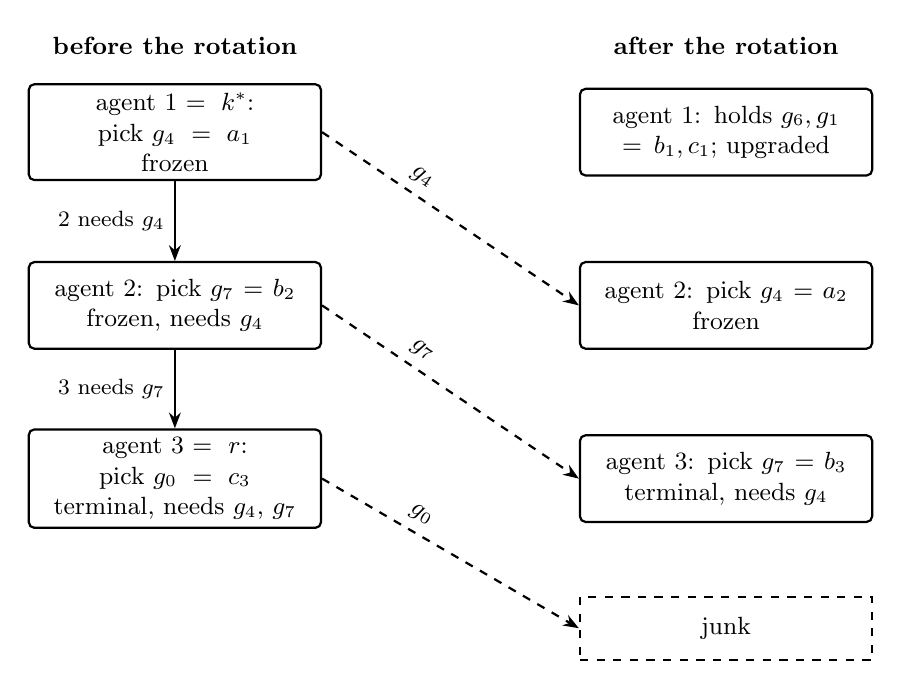
\begin{tikzpicture}[font=\small,
  ag/.style={draw, thick, rounded corners=2pt, align=center, text width=3.5cm, minimum height=1.1cm, inner sep=3pt},
  need/.style={-{Stealth[length=2mm]}, thick},
  move/.style={-{Stealth[length=2mm]}, thick, dashed}]
\node[font=\small\bfseries] at (0,1.1) {before the rotation};
\node[font=\small\bfseries] at (7,1.1) {after the rotation};
\node[ag] (b1) at (0,0) {agent 1 $=k^*$: pick $g_4=a_1$\\frozen};
\node[ag] (b2) at (0,-2.2) {agent 2: pick $g_7=b_2$\\frozen, needs $g_4$};
\node[ag] (b3) at (0,-4.4) {agent 3 $=r$: pick $g_0=c_3$\\terminal, needs $g_4$, $g_7$};
\draw[need] (b1) -- node[left, align=right, font=\footnotesize]{2 needs $g_4$} (b2);
\draw[need] (b2) -- node[left, align=right, font=\footnotesize]{3 needs $g_7$} (b3);
\node[ag] (a1) at (7,0) {agent 1: holds $g_6,g_1$\\$=b_1,c_1$; upgraded};
\node[ag] (a2) at (7,-2.2) {agent 2: pick $g_4=a_2$\\frozen};
\node[ag] (a3) at (7,-4.4) {agent 3: pick $g_7=b_3$\\terminal, needs $g_4$};
\node[draw, thick, dashed, align=center, inner sep=3pt, text width=3.5cm, minimum height=0.8cm] (jk) at (7,-6.3) {junk};
\draw[move] (b1.east) -- node[pos=0.35, above, sloped]{$g_4$} (a2.west);
\draw[move] (b2.east) -- node[pos=0.35, above, sloped]{$g_7$} (a3.west);
\draw[move] (b3.east) -- node[pos=0.35, above, sloped]{$g_0$} (jk.west);
\end{tikzpicture}
\caption{The rotation of Example~\ref{ex:rot}. Left: the need chain $k^*=1\to2\to3=r$ in block~2; each solid arrow points from an agent to an agent that needs its pick. Right: after the rotation, each pick has moved one step down the chain (dashed arrows), $k^*$ holds its $b$ and $c$, and $r$'s old pick has become junk. Agent~0, in block~1, is not drawn.}\label{fig:rot}
\end{figure}

\section{Correctness}\label{sec:correct}

This section proves that Stage L always returns an \efxz{} allocation with at most one bundle of more than two goods. We prove more than K3ALG needs: the results hold for \emph{every} order of Phase 1 with R1 priority, every order of the upgrades and every need chain used by the rotation. This family of runs is construction \LBp{} (Theorem~\ref{thm:C}); K3ALG's smallest-index choices are one member of it, and its tie-breaking plays no role in correctness. Figure~\ref{fig:proofmap} shows how the results depend on each other. Readers who consult the repository's written proof (\file{proofs/lb_last_step.md} of~\cite{Repo}) will find Theorems~\ref{thm:sound}, \ref{thm:A}, \ref{thm:B} and~\ref{thm:C} there as Theorems~1$'$, A, B and~C, and Lemma~\ref{lem:owner} as Lemma~1.

\begin{figure}[tbp]
\centering
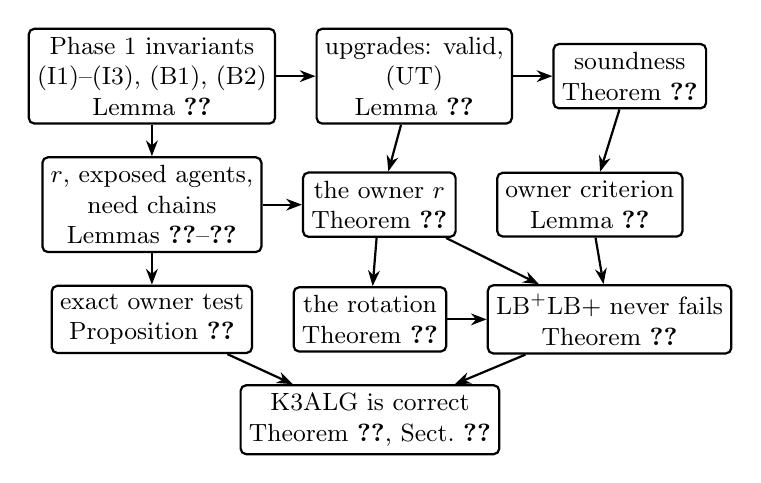
\begin{tikzpicture}[font=\small, node distance=4mm and 5mm,
  res/.style={draw, thick, rounded corners=2pt, align=center, inner sep=3pt, minimum height=7mm},
  arr/.style={-{Stealth[length=2mm]}, thick}]
\node[res] (inv) {Phase 1 invariants\\(I1)--(I3), (B1), (B2)\\Lemma~\ref{lem:inv}};
\node[res, right=of inv] (up) {upgrades: valid,\\(UT)\\Lemma~\ref{lem:upgrades}};
\node[res, right=of up] (sound) {soundness\\Theorem~\ref{thm:sound}};
\node[res, below=of inv] (r) {$r$, exposed agents,\\need chains\\Lemmas~\ref{lem:r}--\ref{lem:count}};
\node[res, right=of r] (A) {the owner $r$\\Theorem~\ref{thm:A}};
\node[res, right=of A] (own) {owner criterion\\Lemma~\ref{lem:owner}};
\node[res, below=of r] (O) {exact owner test\\Proposition~\ref{prop:O}};
\node[res, right=of O] (B) {the rotation\\Theorem~\ref{thm:B}};
\node[res, right=of B] (C) {\LBp{} never fails\\Theorem~\ref{thm:C}};
\node[res, below=of B] (K) {K3ALG is correct\\Theorem~\ref{thm:algo}, Sect.~\ref{sec:k3correct}};
\draw[arr] (inv) -- (up); \draw[arr] (up) -- (sound); \draw[arr] (inv) -- (r); \draw[arr] (r) -- (A);
\draw[arr] (up) -- (A); \draw[arr] (r) -- (O); \draw[arr] (A) -- (B); \draw[arr] (own) -- (C);
\draw[arr] (sound) -- (own); \draw[arr] (A) -- (C); \draw[arr] (B) -- (C); \draw[arr] (O) -- (K); \draw[arr] (C) -- (K);
\end{tikzpicture}
\caption{How the results of Section~\ref{sec:correct} depend on each other. Theorems~\ref{thm:target} and~\ref{thm:D} follow from Theorem~\ref{thm:C} with peeling (Section~\ref{sec:thmC}).}\label{fig:proofmap}
\end{figure}

\subsection{Invariants of Phase 1}\label{sec:inv}

\begin{lemma}[Phase 1]\label{lem:inv}
In every run of Phase 1 (any order for (I1) and (I2); an order with R1 priority for the rest):
\begin{enumerate}
\item[(I1)] If $g\in R_i$ and $g\succ_i Y_i$ (or $Y_i=\none$), then $g$ was picked before $i$'s turn.
\item[(I2)] If $g\in R_i$ is never picked, then $Y_i\ne\none$ and $Y_i\succ_i g$.
\item[(I3)] If all of $R_i$ is still unpicked at $i$'s turn, then $i$ is processed in an insertion step, so it is a leader.
\item[(B1)] When a block starts, every unprocessed agent still has all its goods unpicked.
\item[(B2)] If $g\in R_j$ and $g\succ_j Y_j$ (or $Y_j=\none$), then $g$ was picked by an agent processed before $j$ \emph{in $j$'s block}.
\end{enumerate}
\end{lemma}

\begin{proof}
(I1) At its turn, $i$ took its favourite good among its unpicked goods (or nothing, if none was left), so every good of $R_i$ it ranks higher was already picked; goods leave $G$ only by being picked.
(I2) The good $g$ was unpicked at $i$'s turn, so $i$ had something to pick and took a good it ranks at least as high as $g$; that good is not $g$, which is never picked.
(I3) An R1 step processes only an agent with at most two of its goods unpicked.
(B1) A block starts with an insertion step, which happens only when no unprocessed agent has at most two goods unpicked.
(B2) By (I1), $g$ was picked before $j$'s turn. Suppose it was picked before $j$'s block started. At that moment $j$ was unprocessed and $g\in R_j$ was already picked, which contradicts (B1). So $g$ was picked after $j$'s block started and before $j$'s turn, by an agent of $j$'s block. \qed
\end{proof}

\noindent In words, (B2) says that everything an agent lost, it lost to earlier agents of its own block. R1 priority enters only through (I3), (B1) and (B2), which Lemmas~\ref{lem:lead} and~\ref{lem:chains} below use.

\subsection{The state after the upgrades is valid}\label{sec:valid}

\begin{lemma}[upgrades]\label{lem:upgrades}
Let $Y$ be the picks of a run of Phase 1, and run the upgrade loop in any order. When it stops, $(Y,U)$ is a valid pre-allocation, and (UT) holds.
\end{lemma}

\begin{proof}
\emph{Pre-allocation.} Picks are distinct goods of the pickers. Each upgraded $u$ has $Y_u=b_u$, and $c_u$ was junk when $u$ was upgraded and was then removed from the junk, so the goods $c_u$ are distinct and are nobody's pick.

\emph{(V1).} The junk is a subset of the leftover goods $J_0$. Let $g\in J_0$ and let $i\notin U$ value $g$. By (I2), $Y_i\succ_i g$, so $g\notin N_i$. Hence no leftover good is needed alone, for any $U$.

\emph{(V2).} For $u\in U$, the good $c_u$ is a leftover good, so $c_u\notin\NA$ by the argument for (V1). When $u$ was upgraded, $b_u\notin\NA$ for the set $U$ of that moment. Later upgrades only remove agents' needs from the union $\NA$, so $b_u\notin\NA$ still holds at the end.

\emph{(UT)} is the stopping condition of the loop. \qed
\end{proof}

\noindent In Lean: \lean{EFX.LB.upFinal_valid}. In a valid pre-allocation, every good $g\in\NA$ is the pick of an agent outside $U$: it is not junk by (V1), and it is not $b_u$ or $c_u$ by (V2). That agent's pick is in $\NA$, so it is frozen.

\subsection{Soundness of completions}\label{sec:sound}

\begin{theorem}[soundness]\label{thm:sound}
Let $(Y,U)$ be a valid pre-allocation, and let $X$ be a completion of it, without owner or with an owner $o$, that satisfies the owner constraint (OC). Then $X$ is \efxz{} for every balanced valuation consistent with the rankings, and every bundle except the owner's has at most two goods.
\end{theorem}

\begin{proof}
\emph{Sizes.} A frozen agent other than the owner holds its pick, one good. An upgraded agent other than the owner holds $\{b_i,c_i\}$. A terminal other than the owner holds its base and at most $\capa(i)$ junk goods, and $|\base(i)|+\capa(i)=2$. So only $X_o$ can have more than two goods.

\emph{Bundles of two or more goods contain no good needed alone.} Let $|X_j|\ge2$. Then $j$ is not frozen (unless it is the owner, which is never frozen), so $X_j$ consists of: $j$'s pick if $j$ is a terminal, which is not in $\NA$ by the definition of a terminal; or $b_j$ and $c_j$ if $j\in U$, which are not in $\NA$ by (V2); and junk goods, which are not in $\NA$ by (V1). So $X_j\cap\NA=\emptyset$.

\emph{Each agent is safe.} Fix an agent $i$ and another bundle $X_j$. If $|X_j|\le1$, its threat is $0$ (Lemma~\ref{lem:threat}(a)). So let $|X_j|\ge2$; then $X_j\cap\NA=\emptyset$. Let $h\in X_j$.
\begin{itemize}
\item \emph{$i\in U$.} Then $X_i\supseteq\{b_i,c_i\}$, so $X_j$ meets $R_i$ at most in $a_i$, and $v_i(X_j\setminus\{h\})\le v_i(a_i)\le v_i(b_i)+v_i(c_i)\le v_i(X_i)$, by balance.
\item \emph{$i\notin U$ and $Y_i=\none$.} Then $R_i=N_i\subseteq\NA$, so $X_j$ contains no good of $R_i$, and $v_i(X_j\setminus\{h\})=0\le v_i(X_i)$.
\item \emph{$i\notin U$ with a pick.} A good of $R_i\cap X_j$ is not in $N_i\subseteq\NA$, and it is not $Y_i$, which is in $X_i$. So $i$ ranks it below $Y_i$, and by consistency it is worth at most $v_i(Y_i)\le v_i(X_i)$. If $R_i\cap X_j$ has at most one good, then $v_i(X_j\setminus\{h\})\le v_i(X_j)\le v_i(Y_i)\le v_i(X_i)$. Otherwise $R_i\cap X_j$ consists of two goods ranked below $Y_i$, which forces $Y_i=a_i$ and $R_i\cap X_j=\{b_i,c_i\}$. If $|X_j|=2$, then $X_j=\{b_i,c_i\}$, and $X_j\setminus\{h\}$ is one of these goods, worth at most $v_i(b_i)\le v_i(a_i)\le v_i(X_i)$. If $|X_j|\ge3$, then $j=o$, and $i\notin U$, $i\ne o$, $Y_i=a_i$, $\{b_i,c_i\}\subseteq X_o$: exactly what (OC) excludes. \qed
\end{itemize}
\end{proof}

\noindent The proof uses only agent $i$'s own ranking and balance, so the output depends on the values only through the rankings. It does not cite Lemma~\ref{lem:L5}. In Lean: \lean{EFX.LB.Valid.sound}.

\subsection{The owner criterion}\label{sec:ownercrit}

\begin{lemma}[owner criterion]\label{lem:owner}
Let $(Y,U)$ be valid. (a) If $\omega\le0$, a completion without owner exists, and it satisfies (OC). (b) If $\omega\ge1$ and $o$ is a valid owner with the set $H$, then every completion with owner $o$ that puts every good of $H$ into some slot (that is, $H\subseteq\bigcup_iC_i$) satisfies (OC), and such a completion exists.
\end{lemma}

\begin{proof}
(a) If $|J|\le S$, the junk can be split into sets $C_i$ of at most $\capa(i)$ goods; (OC) is vacuous without owner.
(b) \emph{Existence.} The terminals other than $o$ have $S-\capa(o)\ge|H|$ slots in all, so the goods of $H$ fit into them; the rest of the junk may fill further slots or go to $o$.
\emph{(OC).} Suppose some $x\notin U$, $x\ne o$, with $Y_x=a_x$, has $\{b_x,c_x\}\subseteq X_o=\base(o)\cup(J\setminus C)$, where $C=\bigcup_iC_i$. Then $\{b_x,c_x\}\subseteq J\cup\base(o)$, so $x\in E_o$, and $H$ contains a good $h$ of $\{b_x,c_x\}$. But $h\in H\subseteq C$, so $h$ is junk placed in a slot: it is neither in $J\setminus C$ nor in $\base(o)$, whose goods are not junk. So $h\notin X_o$, a contradiction. \qed
\end{proof}

\noindent K3ALG's $\Complete(o,H)$ is such a completion whenever $H$ consists of junk goods, meets every pair $\{b_x,c_x\}$ with $x\in E_o$, and has at most $S-\capa(o)$ entries: the first $|H|$ entries of the list $L$ lie within the windows of the agents other than $o$, whose total length is $S-\capa(o)$, so every good of $H$ is placed in a slot. Without owner and with $|J|\le S$, $L$ lists the junk without repetition and every good of it is placed. In Lean: \lean{EFX.LB.complete_some} and \lean{EFX.LB.complete_none}.

\subsection{The candidate owner and exposed agents}\label{sec:rexp}

From now on, until Proposition~\ref{prop:O}, fix a run of Phase 1 with R1 priority and of the upgrades, let $(Y,U)$ be the resulting valid pre-allocation (Lemma~\ref{lem:upgrades}), and assume $\omega\ge1$.

\begin{lemma}[the candidate $r$]\label{lem:r}
(A0) Some agent is not upgraded; let $r$ be the last processed agent that is not upgraded. (A1) $r$ is a terminal. (A2) Every agent processed after $r$ is upgraded, and $r$ lies in the last block.
\end{lemma}

\begin{proof}
(A0) The first processed agent is a leader, so it picks its top $a$, while every upgraded agent picked its $b$.
(A1) If $Y_r=\none$, then $r$ is a terminal by definition. Otherwise suppose $Y_r\in\NA$: some $j\notin U$ needs $Y_r$. Then $j\ne r$ (an agent does not need its own pick), and by (I1) $Y_r$ was picked before $j$'s turn; it was picked at $r$'s turn, so $j$ was processed after $r$. As $j\notin U$, this contradicts the choice of $r$. So $r$ is not frozen.
(A2) The first claim is the choice of $r$. The leader of any block after $r$'s would pick its top and so would not be upgraded; hence there is no such block. \qed
\end{proof}

\noindent Let $B^*$ denote $r$'s block. (That it is the last block is not needed below.) In Lean: \lean{EFX.LB.lastOut_exists}, \lean{EFX.LB.lastOut_terminal}.

\begin{lemma}[exposed agents are leaders]\label{lem:lead}
Let $x\in E_r$. Then $x$ was processed before $r$, $x$ is a leader, and $\pi_x\ne\emptyset$. Consequently each block contains at most one agent of $E_r$; in particular $|E_r\cap B^*|\le1$.
\end{lemma}

\begin{proof}
As $x\notin U$ and $x\ne r$, $x$ was processed before $r$ by (A2). At $x$'s turn, $a_x=Y_x$ was unpicked, since $x$ picked it; every junk good was unpicked, since junk is never picked; and $Y_r$ was unpicked, since $r$ picked it later. As $\{b_x,c_x\}\subseteq J\cup\base(r)=J\cup\{Y_r\}$, all of $R_x$ was unpicked at $x$'s turn, and $x$ is a leader by (I3). A block has only one leader. Finally, $b_x\ne c_x$, so at most one of them is $Y_r$, and the other is junk: $\pi_x\ne\emptyset$. \qed
\end{proof}

\noindent In Lean: \lean{EFX.LB.exposed_lead}.

\begin{lemma}[need chains]\label{lem:chains}
Let $x$ be frozen. Then there is a need chain from $x$, and every need chain from $x$ consists of agents of $x$'s block, each processed after the previous one. So every frozen agent $x$ has a terminal $\tau(x)$ in its block that ends a need chain from $x$; for a terminal $x$ let $\tau(x)=x$. In both cases $\capa(\tau(x))\ge1$.
\end{lemma}

\begin{proof}
If $x$ is frozen, some $j\notin U$ needs $Y_x$, and $j\ne x$. By (B2), $Y_x$ was picked by an agent processed before $j$ in $j$'s block; that agent is $x$, the picker of $Y_x$. So $j$ lies in $x$'s block and is processed after $x$. If $j$ is frozen, repeat from $j$. Each step moves strictly later in the processing order, so the agents are distinct, and the process stops, at a terminal, within $x$'s block. The same argument shows that any need chain from $x$ stays in $x$'s block. A terminal has $\capa\ge1$. \qed
\end{proof}

\noindent In Lean: \lean{EFX.LB.chainEnd_spec}. The next lemma is the heart of the argument; Figure~\ref{fig:count} illustrates it.

\begin{lemma}[counting]\label{lem:count}
The terminals $\tau(x)$, for $x\in E_r\setminus B^*$, are pairwise distinct, lie outside $B^*$, and differ from $r$. Hence
\[
  S-\capa(r)\ \ge\ |E_r\setminus B^*|\ \ge\ |E_r|-1 .
\]
\end{lemma}

\begin{proof}
By Lemma~\ref{lem:lead}, different agents of $E_r$ lie in different blocks, and by Lemma~\ref{lem:chains}, $\tau(x)$ lies in $x$'s block. So the terminals $\tau(x)$, $x\in E_r\setminus B^*$, lie in pairwise different blocks other than $B^*$; in particular they are distinct and none is $r\in B^*$. Each has at least one slot, so the terminals other than $r$ have at least $|E_r\setminus B^*|$ slots. Finally $|E_r\cap B^*|\le1$ by Lemma~\ref{lem:lead}. \qed
\end{proof}

\begin{figure}[tbp]
\centering
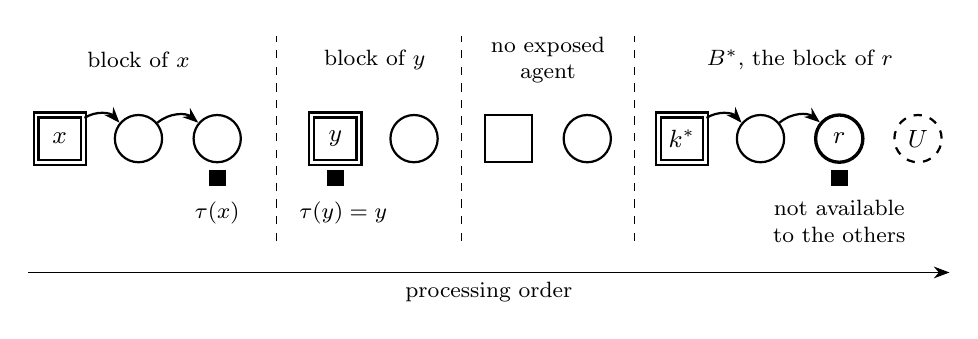
\begin{tikzpicture}[font=\small,
  ldr/.style={draw, thick, minimum size=6mm, inner sep=1pt},
  exl/.style={draw, thick, double, double distance=1pt, minimum size=6mm, inner sep=1pt},
  ag/.style={draw, thick, circle, minimum size=6mm, inner sep=1pt},
  slot/.style={draw, fill=black, minimum size=2mm, inner sep=0pt},
  arr/.style={-{Stealth[length=2mm]}, thick},
  lab/.style={font=\footnotesize, align=center}]
% block of x: x frozen, chain to tau(x)
\node[exl] (x1) at (0,0) {$x$};
\node[ag] (y1) at (1.0,0) {};
\node[ag] (t1) at (2.0,0) {};
\node[slot] at ($(t1)+(0,-0.5)$) {};
\draw[arr] (x1) to[bend left=40] (y1); \draw[arr] (y1) to[bend left=40] (t1);
\node[lab] at (1.0,1.0) {block of $x$};
\node[lab] at (2.0,-0.95) {$\tau(x)$};
\draw[dashed] (2.75,-1.3) -- (2.75,1.3);
% block of y: y is a terminal
\node[exl] (x2) at (3.5,0) {$y$};
\node[slot] at ($(x2)+(0,-0.5)$) {};
\node[ag] (y2) at (4.5,0) {};
\node[lab] at (4.0,1.0) {block of $y$};
\node[lab] at (3.6,-0.95) {$\tau(y)=y$};
\draw[dashed] (5.1,-1.3) -- (5.1,1.3);
% a block without exposed agent
\node[ldr] (z3) at (5.7,0) {};
\node[ag] (w3) at (6.7,0) {};
\node[lab] at (6.2,1.0) {no exposed\\agent};
\draw[dashed] (7.3,-1.3) -- (7.3,1.3);
% B*
\node[exl] (k) at (7.9,0) {$k^*$};
\node[ag] (m) at (8.9,0) {};
\node[ag, very thick] (r) at (9.9,0) {$r$};
\node[slot] at ($(r)+(0,-0.5)$) {};
\node[ag, dashed] (u) at (10.9,0) {$U$};
\draw[arr] (k) to[bend left=40] (m); \draw[arr] (m) to[bend left=40] (r);
\node[lab] at (9.4,1.0) {$B^*$, the block of $r$};
\node[lab] at (9.9,-1.05) {not available\\to the others};
\draw[-{Stealth[length=2mm]}, thin] (-0.4,-1.7) -- node[below, font=\footnotesize]{processing order} (11.3,-1.7);
\end{tikzpicture}
\caption{The counting of Lemma~\ref{lem:count} and Theorem~\ref{thm:A}. Squares are leaders, circles other agents; double borders mark agents exposed for $r$, and black squares mark slots. Exposed agents are leaders (Lemma~\ref{lem:lead}), so they lie in different blocks. Each exposed agent outside $B^*$ reaches a terminal with a slot by a need chain inside its own block (arrows; Lemma~\ref{lem:chains}). Only the exposed leader $k^*$ of $B^*$ may lack such a slot: when all its need chains end at $r$ and no two exposed agents share a junk good, we are in the bad case. Agents processed after $r$ are upgraded.}\label{fig:count}
\end{figure}

\subsection{The owner $r$}\label{sec:thmA}

\begin{theorem}[the owner $r$]\label{thm:A}
Let $(Y,U)$ be the state after a run of Phase 1 with R1 priority and of the upgrades, with $\omega\ge1$. Then $r$ is a valid owner, unless the following \emph{bad case} holds:
\begin{enumerate}
\item[(i)] $r$'s block $B^*$ contains an agent $k^*$ exposed for $r$, and $k^*$ is frozen;
\item[(ii)] every need chain from $k^*$ ends at $r$; and
\item[(iii)] the sets $\pi_x$, $x\in E_r$, are pairwise disjoint.
\end{enumerate}
\end{theorem}

\begin{proof}
Let $H$ consist of one good of each set $\pi_x$ ($x\in E_r$; these sets are nonempty by Lemma~\ref{lem:lead}), choosing a common good when two of the sets meet; so $|H|\le|E_r|$, and $|H|\le|E_r|-1$ if two sets meet. $H$ is a set of junk goods meeting every $\pi_x$, so $r$ is a valid owner as soon as $|H|\le S-\capa(r)$. We use Lemma~\ref{lem:count}.
\begin{itemize}
\item If $E_r\cap B^*=\emptyset$, then $|H|\le|E_r|=|E_r\setminus B^*|\le S-\capa(r)$.
\item Otherwise $E_r\cap B^*=\{k^*\}$ for one agent $k^*$ (Lemma~\ref{lem:lead}), $k^*\ne r$ because $r\notin E_r$, and $|E_r\setminus B^*|=|E_r|-1$.
\begin{itemize}
\item If $k^*$ is a terminal, or some need chain from $k^*$ ends at a terminal other than $r$, then that terminal, $\tau(k^*)$, lies in $B^*$ and differs from $r$ and from all the terminals $\tau(x)$, $x\in E_r\setminus B^*$, which lie outside $B^*$. It has a slot, so $S-\capa(r)\ge|E_r|\ge|H|$.
\item If two of the sets $\pi_x$ meet, then $|H|\le|E_r|-1=|E_r\setminus B^*|\le S-\capa(r)$.
\end{itemize}
\end{itemize}
If none of these cases applies, then $k^*$ exists, is not a terminal, and is not upgraded (it is exposed), so it is frozen; every need chain from $k^*$ ends at $r$; and the sets $\pi_x$ are pairwise disjoint. This is the bad case. \qed
\end{proof}

\noindent In Lean: \lean{EFX.LB.theoremA_invalid} (if $r$ is not a valid owner, the bad case holds). Example~\ref{ex:owner} is the first case of the proof, and Example~\ref{ex:rot} is the bad case.

\subsection{The rotation}\label{sec:thmB}

Assume the bad case, and write $k=k^*$. Fix any need chain $x_0,x_1,\dots,x_t$ from $x_0=k$, with $t\ge1$; one exists by Lemma~\ref{lem:chains}, and it ends at $x_t=r$ by (ii). Define the rotated pre-allocation $P'=(Y',U')$:
\begin{itemize}
\item $Y'_{x_s}=Y_{x_{s-1}}$ for $1\le s\le t$: every later agent of the chain takes the good it needed from its predecessor;
\item $Y'_k=b_k$ and $U'=U\cup\{k\}$: agent $k$ gives up $a_k$ and takes $b_k$ and $c_k$;
\item every other agent keeps its pick and its upgrade status.
\end{itemize}
Let $W=J\cup\{Y_r\}$ (just $J$ if $Y_r=\none$). Since $k\in E_r$, $\{b_k,c_k\}\subseteq W$. The new junk is $J'=W\setminus\{b_k,c_k\}$: the pick of $r$, if any, is released, and every pick of $P$ other than $Y_r$ is still a pick in $P'$, possibly of another agent of the chain. Primes denote the notions of $P'$: $N'_i$, $\NA'$, $\capa'$, $S'$, $\omega'$ and $E'_k$ (exposure for the owner $k$ in $P'$). Note that $J'\cup\{b_k,c_k\}=W$.

\begin{theorem}[the rotation]\label{thm:B}
In the bad case, $P'$ is a valid pre-allocation with $\NA'\subseteq\NA$. If $\omega'\le0$, it has a completion without owner. If $\omega'\ge1$, then every $x\in E'_k$ has $\pi'_x=\{b_x,c_x\}\cap J'\ne\emptyset$ and $|E'_k|\le S'$; in particular $k$ is a valid owner of $P'$, and $\HitSet(E'_k)$ is a witness.
\end{theorem}

\begin{proof}
(a) \emph{$P'$ is a pre-allocation.} Each $x_s$ ($s\ge1$) needed $Y_{x_{s-1}}$, so $Y'_{x_s}\in R_{x_s}$. The picks of $P'$ are the picks of $P$ other than $Y_r$, rearranged along the chain, together with $b_k$; since $b_k\in W$, it is not a pick of $P$ other than $Y_r$, so no good is picked twice. Also $c_k\in W$ and $c_k\ne b_k$, so $c_k$ is not a pick of $P'$; and it differs from every $c_u$, $u\in U$, which is not in $W$. Finally $Y'_k=b_k$, as the definition requires for $k\in U'$.

(b) \emph{$\NA'\subseteq\NA$.} For $s\ge1$, $x_s$ ranks $Y'_{x_s}$ above $Y_{x_s}$ (or $Y_{x_s}=\none$), so $N'_{x_s}\subseteq N_{x_s}$. Agent $k$ had $N_k=\emptyset$, since $Y_k=a_k$, and is now in $U'$. Every other agent keeps its needs.

(c) \emph{Validity.} (V1): $J'\subseteq W$, $J\cap\NA=\emptyset$ by (V1) for $P$, and $Y_r\notin\NA$ by (A1); so $J'\cap\NA'=\emptyset$. (V2): for $u\in U$, $b_u,c_u\notin\NA\supseteq\NA'$; for $k$, $b_k,c_k\in W$, and $W\cap\NA=\emptyset$ as just shown.

(d) \emph{Terminals outside $B^*$ survive.} The chain lies in $B^*$ (Lemma~\ref{lem:chains}). Let $x$ be a terminal of $P$ outside $B^*$. It keeps its pick and stays outside $U'$, and $Y'_x=Y_x\notin\NA\supseteq\NA'$, so it is a terminal of $P'$ with the same number of slots.

(e) \emph{$E'_k\subseteq E_r\setminus\{k\}$.} By definition $E'_k$ is the set of $x\notin U'$, $x\ne k$, with $Y'_x=a_x$ and $\{b_x,c_x\}\subseteq J'\cup\{b_k,c_k\}=W$. Let $x\in E'_k$.
\begin{itemize}
\item If $x$ is not on the chain, then $Y_x=Y'_x=a_x$, $x\notin U$, $x\ne r$, and $\{b_x,c_x\}\subseteq W=J\cup\base(r)$. So $x\in E_r$.
\item $x=x_s$ with $1\le s\le t-1$ is impossible. Since $a_x=Y'_x\succ_x Y_x$, the old pick $Y_x$ is $b_x$ or $c_x$; but $Y_x$ is a pick of $P$ other than $Y_r$, so $Y_x\notin W$, contradicting $\{b_x,c_x\}\subseteq W$.
\item $x=r$ is impossible. Since $r$ needs $Y_{x_{t-1}}$, $Y_r\ne a_r$, so there are three cases. If $Y_r=\none$, then $b_r\in N_r$ was picked by another agent (I1), so $b_r\notin W$. If $Y_r=c_r$, the same holds for $b_r$. If $Y_r=b_r$, then (UT) applies to $r$: $r\notin U$, and $b_r\notin\NA$ by (A1), so $c_r\notin J$; and $c_r\ne Y_r$, so $c_r\notin W$. In each case $\{b_r,c_r\}\not\subseteq W$.
\end{itemize}

(f) \emph{Every exposed pair has a junk good.} Let $x\in E'_k$, and suppose $\{b_x,c_x\}\subseteq\{b_k,c_k\}$, so the two pairs are equal. By (e), $x\in E_r\setminus\{k\}$, and then $\pi_x=\{b_x,c_x\}\cap J=\{b_k,c_k\}\cap J=\pi_k$, which is nonempty (Lemma~\ref{lem:lead}); this contradicts the disjointness (iii) of the bad case. So $\{b_x,c_x\}$ has a good outside $\{b_k,c_k\}$, which lies in $J'$ because $\{b_x,c_x\}\subseteq J'\cup\{b_k,c_k\}$: $\pi'_x\ne\emptyset$.

(g) \emph{Counting.} By (e), $|E'_k|\le|E_r|-1=|E_r\setminus B^*|$, since $E_r\cap B^*=\{k\}$. The terminals $\tau(x)$, $x\in E_r\setminus B^*$, are distinct and lie outside $B^*$ (Lemma~\ref{lem:count}), so by (d) they are terminals of $P'$ with at least one slot each. Hence $|E'_k|\le S'=S'-\capa'(k)$, as $k\in U'$ has no slots.

Finally, if $\omega'\le0$, Lemma~\ref{lem:owner}(a) applies. If $\omega'\ge1$, then one junk good from each $\pi'_x$, $x\in E'_k$, forms a set of at most $|E'_k|\le S'-\capa'(k)$ junk goods meeting every exposed pair, so $k$ is a valid owner. The list $\HitSet(E'_k)$ has at most $|E'_k|$ entries, each a junk good (the shared good of the first meeting pair, or $\mathrm{one}(z)\in\pi'_z$, which is junk because $\pi'_z\ne\emptyset$), and it meets every pair. \qed
\end{proof}

\noindent In Lean: \lean{EFX.LB.theoremB}, for any need chain. Figure~\ref{fig:rot} shows a rotation, and Example~\ref{ex:rot} illustrates (e)--(g): after the rotation, only agent~$0\in E_r\setminus B^*$ is exposed for $k^*$, and the terminals outside $B^*$ keep their slots.

\subsection{Construction \LBp{} never fails}\label{sec:thmC}

\emph{Construction \LBp{}} is the following family of runs on an instance in which every agent values exactly three goods, ranked, and is balanced.
\begin{enumerate}
\item Run Phase 1 in any order with R1 priority, then the upgrades in any order.
\item If $\omega\le0$, return any completion without owner.
\item Otherwise, if $r$ is a valid owner, return any completion with owner $r$ that satisfies (OC).
\item Otherwise rotate along any need chain from $k^*$ to $r$. If $\omega'\le0$, return any completion of $P'$ without owner; otherwise return any completion of $P'$ with owner $k^*$ that satisfies (OC).
\end{enumerate}

\begin{theorem}[\LBp{} never fails]\label{thm:C}
For every instance in which every agent values exactly three goods and is balanced, and for every run of \LBp{}, an output exists (every step above is possible), and every output is a complete allocation that is \efxz{} for every balanced valuation consistent with the rankings, in which at most one bundle has more than two goods.
\end{theorem}

\begin{proof}
Step~1 gives a valid pre-allocation (Lemma~\ref{lem:upgrades}). In step~2, a completion without owner exists (Lemma~\ref{lem:owner}(a)). In step~3, a completion with owner $r$ satisfying (OC) exists (Lemma~\ref{lem:owner}(b)). In step~4, $r$ is not a valid owner, so the bad case holds (Theorem~\ref{thm:A}): $k^*$ exists, a need chain from $k^*$ exists, and every such chain ends at $r$. By Theorem~\ref{thm:B}, $P'$ is valid, and either $\omega'\le0$ and a completion without owner exists, or $k^*$ is a valid owner of $P'$ and a completion with owner $k^*$ satisfying (OC) exists (Lemma~\ref{lem:owner}(b)). Every returned completion is of a valid pre-allocation and satisfies (OC), vacuously when there is no owner, so Theorem~\ref{thm:sound} applies. \qed
\end{proof}

\noindent In Lean: \lean{EFX.LB.lbPlusRun_sound} (every output is sound, over all runs), \lean{EFX.LB.lbPlusOut_exists} (an output exists) and \lean{EFX.LB.lbPlusOut_exists_chain} (in the rotation branch, every need chain from $k^*$ to $r$ gives one).

\begin{proof}[of Theorem~\ref{thm:D}]
Rank each agent's three goods by value, ties by index; the valuation is consistent with these rankings and balanced. Run \LBp{} (for instance K3ALG's Stage L, which is one of its runs). By Theorem~\ref{thm:C}, the output is \efxz{} for this valuation, and at most one bundle has more than two goods. The argument never uses that values are integers. \qed
\end{proof}

\begin{proof}[of Theorem~\ref{thm:target}]
By induction on the number of agents $n\ge1$. With one agent, give it everything. With no goods, give everyone nothing. Otherwise, if rule R1 applies to some agent $i$, with bundle $P$ ($P=\{p\}$ or $\emptyset$), the instance without $i$ and $P$ is again $3$-relevant and has $n-1\ge1$ agents, so it has an \efxz{} allocation by induction, and Lemma~\ref{lem:peel} extends it. If R1 applies to no agent, then by Lemma~\ref{lem:R1fail} every agent values exactly three goods and is strictly balanced, and Theorem~\ref{thm:D} applies. \qed
\end{proof}

\noindent The Lean proofs of Theorems~\ref{thm:target} and~\ref{thm:D} are over natural-number values, \lean{EFX.target} and \lean{EFX.LB.corollaryD}; Lemma~\ref{lem:L12} transfers them to any linearly ordered cancellative commutative monoid (\lean{EFX.target_ordered}, \lean{EFX.corollaryD_ordered}; Section~\ref{sec:lean}). The Lean proof of Theorem~\ref{thm:target} goes through the reduction to cores of Section~\ref{sec:cert} (\lean{EFX.core_reduction}), which also removes goods nobody values and peels by rule R2; the proof above shows that rule R1 alone suffices, which is the route K3ALG takes and whose Lean form is \lean{EFX.K3.reduce_sound}.

\subsection{The owner test is exact}\label{sec:propO}

To apply Theorem~\ref{thm:C}, an algorithm must decide whether $r$ is a valid owner. In general, deciding whether some set of at most $s$ junk goods meets every set $\pi_x$ is a minimum hitting set problem; since each $\pi_x$ has at most two goods, it is vertex cover on the graph whose vertices are the junk goods and whose edges are the sets $\pi_x$, which is NP-hard in general. For the particular owner $r$ the counting of Lemma~\ref{lem:count} makes it easy.

\begin{proposition}[the owner test]\label{prop:O}
Let $(Y,U)$ be the state after a run of Phase 1 with R1 priority and of the upgrades, with $\omega\ge1$. Then $r$ is a valid owner if and only if
\[
  |E_r|\le S-\capa(r)\qquad\text{or}\qquad\text{two of the sets }\pi_x\ (x\in E_r)\text{ meet.}
\]
In either case $\HitSet(E_r)$ is a witness: it lists junk goods, meets $\pi_x$ for every $x\in E_r$, and has at most $S-\capa(r)$ entries. Consequently, $r$ is a valid owner if and only if $\HitSet(E_r)$ has at most $S-\capa(r)$ entries.
\end{proposition}

\begin{proof}
Let $\tau$ be the smallest number of junk goods that meet every set $\pi_x$, $x\in E_r$. By definition, $r$ is a valid owner if and only if $\tau\le S-\capa(r)$.
\begin{itemize}
\item \emph{$\tau\le|E_r|$, and $\tau\le|E_r|-1$ if and only if two of the sets meet.} All the sets are nonempty (Lemma~\ref{lem:lead}), so one good from each gives $\tau\le|E_r|$. If $g\in\pi_x\cap\pi_y$ for $x\ne y$, then $g$ together with one good from each other set meets all of them, with at most $|E_r|-1$ goods. If the sets are pairwise disjoint, a set meeting all of them contains a different good of each, so $\tau=|E_r|$.
\item \emph{Sufficiency.} If $|E_r|\le S-\capa(r)$, then $\tau\le|E_r|\le S-\capa(r)$. If two sets meet, then $\tau\le|E_r|-1\le S-\capa(r)$ by Lemma~\ref{lem:count}.
\item \emph{Necessity.} If no two sets meet, then $\tau=|E_r|$, so $\tau\le S-\capa(r)$ gives $|E_r|\le S-\capa(r)$.
\item \emph{The witness.} Every entry of $\HitSet(E_r)$ is junk: the shared good $g$ is in $\pi_x\cap\pi_y$, and $\mathrm{one}(z)$ is $b_z$ if $b_z$ is junk and otherwise $c_z$, which is then junk because $\pi_z\ne\emptyset$. The list meets every $\pi_x$ ($x$ and $y$ through $g$, every other $z$ through $\mathrm{one}(z)$), and it has $|E_r|-1$ entries if two sets meet and $|E_r|$ otherwise. By the previous items, in both cases of the condition it has at most $S-\capa(r)$ entries, and if the condition fails it has $|E_r|>S-\capa(r)$ entries. \qed
\end{itemize}
\end{proof}

\noindent In Lean: \lean{EFX.LB.validOwner_iff}, with the counting \lean{EFX.LB.hitSet_fits} and the length \lean{EFX.LB.hitSet_length}. The simpler test ``$|E_r|\le S-\capa(r)$'', one good per exposed agent without sharing, is not enough: it rejects some valid owners outside the bad case, where the rotation's guarantees do not hold (a smallest configuration is recorded in the repository~\cite{Repo}). After the rotation no test is needed, by Theorem~\ref{thm:B}.

\subsection{Correctness of K3ALG}\label{sec:k3correct}

\begin{proof}[of Theorem~\ref{thm:algo}, correctness]
Let every agent value at most three goods. \emph{Stage R} peels agents by rule R1, so by Lemma~\ref{lem:peel} and induction it suffices that Stage L returns an \efxz{} allocation of the agents $A$ and goods $M$ it receives (when Stage R returns directly, what remains is one agent, which takes everything, or no goods, and its allocation is trivially \efxz{}). When Stage L starts, every agent of $A$ values exactly three goods of $M$ and is strictly balanced (Lemma~\ref{lem:R1fail}), and the computed rankings are consistent with the values. We check that Stage L is a run of \LBp{}.
\begin{itemize}
\item Phase 1 serves the first agent with at most two goods left, if any, which is an order with R1 priority; the upgrades run in index order.
\item If $|J|\le S$, it returns a completion without owner (step~2).
\item Otherwise its test $|\HitSet(E_r)|\le S-\capa(r)$ holds exactly when $r$ is a valid owner (Proposition~\ref{prop:O}). If it holds, $\Complete(r,\HitSet(E_r))$ is a completion satisfying (OC) (Proposition~\ref{prop:O} and the remark after Lemma~\ref{lem:owner}): step~3.
\item If the test fails, $r$ is not a valid owner, so the bad case holds (Theorem~\ref{thm:A}). Then $E_r\cap B^*=\{k^*\}$, so the first agent of $E_r$ in $r$'s block is $k^*$. The scan builds a need chain from $k^*$: each appended agent is outside $U$ and needs the pick of the frozen agent before it, all are distinct (they are scanned in order), and while the last agent is frozen, the agent that needs its pick comes later in the order (Lemma~\ref{lem:chains}), so the scan finds it; hence the chain ends at a terminal, which is $r$ by (ii). The rotation is then that of Theorem~\ref{thm:B}. If $|J'|\le S'$, K3ALG completes without owner; otherwise $\HitSet(E'_{k^*})$ is a witness that $k^*$ is a valid owner (Theorem~\ref{thm:B}), and $\Complete(k^*,\HitSet(E'_{k^*}))$ satisfies (OC): step~4.
\end{itemize}
By Theorem~\ref{thm:C}, Stage L's output is \efxz{}. \qed
\end{proof}

\noindent In Lean: \lean{EFX.K3.algo_efx0}, via \lean{EFX.K3.algo_eq_spec} (the counted program computes the specification) and \lean{EFX.K3.algoSpec_efx0}. The two ``impossible'' branches of the listing (no $r$, no $k^*$) are indeed never taken, by Lemma~\ref{lem:r} and Theorem~\ref{thm:A}.

\subsection{The size of the large bundle}\label{sec:size}

\begin{proposition}[size of the large bundle; written, not formalized]\label{prop:size}
Let $(Y,U)$ be a valid pre-allocation of an instance with $n$ agents and $m$ goods in which every agent values exactly three goods. Then $\omega=m-2n+|\NA|$. If $\omega\ge1$, every completion with owner $o$ in which all slots of the terminals other than $o$ are full gives $o$ exactly $\omega+2$ goods.
\end{proposition}

\begin{proof}
In a valid pre-allocation, each good of $\NA$ is the pick of an agent outside $U$, which is then frozen (Section~\ref{sec:valid}), and each frozen agent's pick is in $\NA$; so the frozen agents $F$ satisfy $|F|=|\NA|$. Let $T_1$ and $T_0$ be the terminals with and without a pick. Every good is a pick, a good $c_u$, or junk, so $m=(|U|+|F|+|T_1|)+|U|+|J|$, while $S=|T_1|+2|T_0|$ and $n=|U|+|F|+|T_1|+|T_0|$. Hence
\[
  \omega=|J|-S=m-2|U|-|F|-2|T_1|-2|T_0|=m-2n+|F|=m-2n+|\NA|.
\]
With the other slots full, the owner receives its base and the $|J|-(S-\capa(o))=\omega+\capa(o)$ remaining junk goods, and $|\base(o)|+\capa(o)=2$ for every terminal and every upgraded agent. \qed
\end{proof}

\noindent The rotation does not increase $\NA$ (Theorem~\ref{thm:B}), so it does not enlarge the large bundle. In Example~\ref{ex:owner}, $m-2n+|\NA|=8-8+1=1=\omega$ for the Stage-L instance, and the owner holds $3$ goods.

\begin{remark}[a repeated good]\label{rem:repeat}
K3ALG's completion fills every slot of the terminals other than the owner when $\HitSet$ lists no good twice, and then Proposition~\ref{prop:size} gives the size of its large bundle. A good can be listed twice, and then a slot stays empty and the owner receives more goods; the output is still \efxz{} by Lemma~\ref{lem:owner}. For example, let four agents value $g_0$ at $3$, and agent $i$ also value $g_{2i+1}$ at $4$ and $g_{2i+2}$ at $2$ ($i=0,\dots,3$, nine goods). All four agents are leaders and pick their tops, $\NA=\emptyset$, every agent is a terminal with one slot, $S=4$ and $|J|=5$, so $\omega=1$. The owner is $r=3$, with $E_3=\{0,1,2\}$ and $\HitSet(E_3)=(g_0,g_0)$: the pair of agents $0$ and $1$ shares $g_0$, and agent~$2$'s junk $b$ is $g_0$ again. So $L=(g_0,g_0,g_2,g_4,g_6,g_8)$: agent~$0$ receives $g_0$, agent~$1$'s window holds only the repeated $g_0$, agent~$2$ receives $g_2$, and the owner receives $g_4$, $g_6$ and $g_8$ besides its pick $g_7$: four goods in all, which is $\omega+3$.
\end{remark}

\section{Running Time}\label{sec:time}

This section proves the running-time part of Theorem~\ref{thm:algo} and its corollaries. Section~\ref{sec:owner-time} explains why the owner test is cheap; Section~\ref{sec:leanbound} describes the machine-checked bound and the cost model it is stated in; Sections~\ref{sec:bits} and~\ref{sec:ratreal} give written, not formalized, corollaries for the bit model and for rational and real values; and Section~\ref{sec:finer} separates a finer written bound from measurements of implementations.

\subsection{The owner test in polynomial time}\label{sec:owner-time}

The only step of \LBp{} that looks expensive is the owner test, since for an arbitrary candidate owner it is a vertex-cover question (Section~\ref{sec:propO}). Proposition~\ref{prop:O} removes the issue for the candidate $r$: $r$ is a valid owner if and only if the explicit list $\HitSet(E_r)$ has at most $S-\capa(r)$ entries. Computing $\HitSet(E)$ means finding the first pair of agents of $E$ whose sets $\pi$ share a junk good: $O(|E|^2)$ pair checks, so $O(|E|^2+m)$ steps with a junk flag per good, or $O(|E|^2m)$ as formalized, where membership in $J$ is a list scan. With an index from each junk good to the exposed agents whose pair contains it, $O(|E|+|J|)$ steps suffice. After the rotation no test is needed (Theorem~\ref{thm:B}). Whether the test is hard for an arbitrary owner, on the graphs that arise here, is open; \LBp{} never asks.

\subsection{The machine-checked operation bound}\label{sec:leanbound}

\paragraph{The program and its cost.} In Lean, K3ALG is written in a \emph{cost monad}, \lean{EFX.Timed}: a value of type \texttt{Timed}~$\alpha$ is a value of type $\alpha$ paired with a natural number, the count; \texttt{tick~$k$} adds $k$ to the count, and sequencing adds the counts of the steps actually evaluated. The algorithm is \lean{EFX.K3.algoC}, of type \texttt{Timed}~\texttt{Alloc}, and
\begin{alltt}
def EFX.K3.algo (I : Inst) (hn : 0 < I.n) : I.Alloc :=
  (algoC I hn).val
\end{alltt}
is its value. So the machine-checked bound below is a bound for the very program whose value is the allocation, not for a separately written cost function. Each counted definition has a \emph{value lemma} saying that it computes the corresponding uncounted definition of Section~\ref{sec:correct}'s formalization; for the whole program this is \lean{EFX.K3.algo_eq_spec}.

\begin{theorem}[running time; \texttt{EFX.K3.algoC\_cost}]\label{thm:time}
For every instance with $n\ge1$ agents and $m$ goods, with any natural-number values (no assumption on the number of relevant goods), $\mathtt{(algoC\ I\ hn).cost}\le400(n+m+1)^4$; also $\le6400(n+m)^4$ (\texttt{EFX.K3.algoC\_cost'}).
\end{theorem}

\paragraph{The cost model.} One unit is counted for each of the following:
\begin{itemize}
\item one step of a list traversal (a cell visited by \texttt{map}, \texttt{filter}, \texttt{any}, \texttt{find}, a sum, \texttt{length}, append, \texttt{take}, \texttt{drop}, membership or \texttt{erase}, or by the recursions of Phase~1, the blocks, the need chain, the rotation, the completion and the search for $r$), together with the comparison made there;
\item one comparison of two agents or two goods;
\item one read of an input value $v_i(g)$ (the input is an $n\times m$ matrix);
\item one comparison or addition of two natural numbers, of any size;
\item one read of a \emph{table}: the rankings $a_i,b_i,c_i$, the picks, the blocks, the slots and the output are arrays filled once (\lean{EFX.Timed.mkTable}); filling a table costs the evaluation of its entries plus one unit per entry.
\end{itemize}
Straight-line code with a bounded number of these operations is charged by a single \texttt{tick~$k$}, with $k$ at least that number; for example, sorting one agent's three goods costs \texttt{tick 10} (at most four list cells, three value reads and three comparisons), and computing the rank of a good for an agent costs \texttt{tick 6} (three table reads and three comparisons). Not counted: building pairs, options and list cells that a counted step produces, and matching on them; Boolean connectives on computed Booleans (a constant number per counted step); building closures; and the size of numbers, which Corollary~\ref{cor:bits} accounts for.

\paragraph{The accounting discipline.} Four rules make the count meaningful.
\begin{enumerate}
\item Every list traversal goes through a charged combinator, such as \lean{mapC}, \lean{filterC}, \lean{anyC}, \lean{findC}, \lean{memC}, \lean{eraseC}, \lean{sumMapC} or \lean{lengthC}: one unit per cell visited, plus the cost of the element function. The recursions of Phase~1, the blocks, the chain, the rotation and the completion charge one unit per step.
\item Every call of an uncounted function sits under a \texttt{tick} that bounds its work: \lean{sort3C} is \texttt{tick 10}, \lean{rankC} is \texttt{tick 6}, and \lean{finRangeC}~$k$ is \texttt{tick}~$k$.
\item No recursion over lists runs outside the monad, and each counted definition has a value lemma, so every loop of the specification is a counted loop.
\item Every table is filled once by \lean{mkTable}, and each read costs one unit.
\end{enumerate} The value lemmas and the bound are machine-checked; that each \texttt{tick} and each \texttt{pure} covers the work it stands for is not, and belongs to the trusted base. An auditor should read the \texttt{tick}s and \texttt{pure}s of \texttt{Timed.lean}, \texttt{K3CostLB.lean} and \texttt{K3Cost.lean}; each is annotated with what it counts.

\paragraph{Where the fourth power comes from.} The proof bounds every counted step in terms of one number $N=n+m+1$, which exceeds the length of every list the program builds: agents, upgraded agents (with $k^*$), exposed agents, the chain and the order have at most $n+1$ elements; the remaining goods, the junk and the pools at most $m$; the placement list at most $n+m$. Appendix~\ref{app:cost} lists the bound for each step. The degree-four term comes from the upgrade loop: at most $n$ rounds, each testing up to $n$ candidates, each test deciding whether $b_k\in\NA$ by scanning $n$ agents with a membership test in $U$ ($36N^4$ in all, \lean{EFX.K3.lbUpC_cost}). Stage L costs at most $310N^4$ (\lean{EFX.K3.lbPlusC_cost}), Stage R at most $15N^2$ per round, and the whole program at most $400N^4$.

\subsection{Bit complexity}\label{sec:bits}

The unit-cost model charges one unit for arithmetic on numbers of any size. The next corollary shows that this is harmless here.

\begin{corollary}[bit complexity; written, not formalized]\label{cor:bits}
Let $b$ be the largest bit length of an input value. If each operation of the cost model costs the bit length of its operands, K3ALG takes $O\big((n+m)^4(b+\log(n+m))\big)$ bit operations.
\end{corollary}

\begin{proof}
We read the counted program, which is in the files \texttt{Timed.lean}, \texttt{K3CostLB.lean} and \texttt{K3Cost.lean}. It forms no products. Values enter only in Stage~R and in the computation of the rankings: each is compared with $0$ or with another value of the same agent, and rule R1 compares $v_i(p)$ with $v_i(M\setminus\{p\})$, a sum of values of agent $i$ over the remaining goods. So every number derived from values is a sum of at most $m$ values of one agent, below $m2^b$, and Stage~L reads no values at all. The other numbers are ranks in $\{0,1,2,3\}$, slot counts and their sums (at most $2n$), list lengths (at most $n+m$) and block counters (at most $n$), and agents and goods are indices below $n$ and $m$. So every operand, including table addresses, has $O(b+\log(n+m))$ bits, and each counted operation costs that many bit operations. Multiply by the bound of Theorem~\ref{thm:time}. \qed
\end{proof}

\subsection{Rational and real values}\label{sec:ratreal}

\begin{proof}[of Corollary~\ref{cor:rat}]
Multiply agent $i$'s values by a common denominator of them. This multiplies every sum of $i$'s values by the same positive number, so every comparison between two such sums is preserved, and with it the relevant goods, the \efxz{} condition, and every decision of K3ALG. \qed
\end{proof}

\noindent For real values, the model must say what an algorithm can do with a real number. We use a comparison oracle.

\begin{corollary}[real values; written, not formalized]\label{cor:real}
Suppose every agent positively values at most three goods, and an oracle compares two sums of one agent's real values at unit cost. Then computing the valuations $w$ of Lemma~\ref{lem:L12} and running K3ALG on them takes $O(nm)$ oracle calls and $O((n+m)^4)$ further operations, and the output is \efxz{} for the real values.
\end{corollary}

\begin{proof}
Lemma~\ref{lem:L12} is constructive. For each agent, finding $R_i$ takes $m$ comparisons with $0$. At most six more comparisons determine $w_i$: three to sort the relevant goods, the ties among them, and the comparison of the top with the sum of the other two (Appendix~\ref{app:L12}). The entries of $w$ are at most $5$. K3ALG on $w$ takes $O((n+m)^4)$ operations (Theorem~\ref{thm:time}), with numbers of $O(\log m)$ bits, and its output is \efxz{} for $w$ (Theorem~\ref{thm:algo}), hence for $v$ (Lemma~\ref{lem:L12}). \qed
\end{proof}

\noindent Alternatively, K3ALG can run on real inputs directly. Every decision it makes compares two sums of one agent's values (relevance, the favourite good, rule R1, and the three comparisons of the sort), and Lemma~\ref{lem:L12} answers each such comparison for $v$ as for $w$, so the run on $v$ is the run on $w$ and returns the same allocation. This is also written, not formalized.

\subsection{A finer bound and measurements}\label{sec:finer}

\paragraph{A finer written bound.} Bounding each step by its own parameters instead of $N$ (Appendix~\ref{app:cost}, last column) gives $O(n^4+n^2m)$ operations for the formalized program. This analysis is written, not machine-checked; Lean states only the coarser $400(n+m+1)^4$.

\paragraph{A faster implementation.} A Python implementation of the same algorithm (\texttt{fast} in the repository's \file{k3/k3algo.py}) replaces the naive scans by a heap of the agents to which R1 applies (under $3$-relevance, R1 keeps applying to an agent once it applies), a heap of the agents with a good missing (for Phase~1's order), per-good counters of the agents that rank a good above their pick (for the upgrades), and an index from junk goods to exposed agents (for $\HitSet$). Its written analysis, not formalized, gives $O((n+m)\log n)$ operations after the input is read.

\paragraph{Measurements (evidence, not guarantees).} The following are measurements of implementations, recorded in the repository~\cite{Repo}; they are not part of any theorem.
\begin{itemize}
\item \texttt{fast} returns the same allocation as a literal transcription of the Lean definitions on $200{,}000$ random instances; on $675$ instances both agree with Lean's own evaluation of \lean{EFX.K3.algo}, every Lean output passes a raw \efxz{} check, and every Lean operation count is below the proved bound. The largest count divided by $(n+m+1)^4$ falls from $0.38$ at $n=2$ to $0.002$ at $n=30$, against the factor $400$ of the bound.
\item Median running times of \texttt{fast} (Python~3.11, one CPU, three instances per point), on random instances in which every agent values exactly three goods and is balanced, with $m=1.5n$ (``core'') and $m=2n$ (``core2m''), and on random instances in which each agent values between zero and three goods (``general''), in seconds:
\begin{center}\small
\setlength{\tabcolsep}{4pt}\begin{tabular}{@{}rrrrr@{}}
\toprule
$n$ & core & core2m & general & literal transcription (core2m) \\
\midrule
$80$ & $0.0006$ & $0.0007$ & $0.0004$ & $0.30$ \\
$1{,}000$ & $0.0073$ & $0.0074$ & $0.0051$ & -- \\
$10{,}000$ & $0.082$ & $0.089$ & $0.062$ & -- \\
$100{,}000$ & $1.53$ & $1.58$ & $0.84$ & -- \\
\bottomrule
\end{tabular}
\end{center}
The log--log slopes of \texttt{fast} between consecutive sizes are between $1.0$ and $1.4$, consistent with $O((n+m)\log n)$.
\end{itemize}

\section{The Machine-Checked Proof}\label{sec:lean}

This section describes the Lean~4 formalization~\cite{Repo}: what it covers, what a reader must trust, how to read its main statements, and what it leaves out. Appendix~\ref{app:lean} maps every result of this paper to its Lean names.

\subsection{What is formalized}\label{sec:lean-what}

\begin{itemize}
\item \emph{Theorems~\ref{thm:target} and~\ref{thm:D}}, for natural-number values (\lean{EFX.target}, \lean{EFX.LB.corollaryD}) and for values in any linearly ordered cancellative commutative monoid (\lean{EFX.target_ordered}, \lean{EFX.corollaryD_ordered}).
\item \emph{Theorem~\ref{thm:algo}}: the algorithm, a computable function (\lean{EFX.K3.algo}); its correctness (\lean{EFX.K3.algo_efx0}); and its operation bound, for the counted program whose value is the algorithm (\lean{EFX.K3.algoC_cost}).
\item \emph{Section~\ref{sec:correct}} in full, except Proposition~\ref{prop:size}, and except the remark that $r$ lies in the last block, which no proof uses: the invariants of Phase~1, the validity of the upgrades, soundness, the owner criterion, Lemmas~\ref{lem:r}--\ref{lem:count}, Theorems~\ref{thm:A}, \ref{thm:B} and~\ref{thm:C}, and Proposition~\ref{prop:O}. \LBp{} is formalized both as a relation over all its runs and as a computable function, the one K3ALG uses.
\item \emph{Section~\ref{sec:prelim}}: peeling (rules R1 and R2, and the general Lemma~\ref{lem:peel}); Lemmas~\ref{lem:R1fail}, \ref{lem:junk} and~\ref{lem:L12}; and Corollary~\ref{cor:k2}, as an existence statement. Also the reduction to cores of Section~\ref{sec:cert}.
\item \emph{Examples}: three runs of K3ALG checked by \texttt{decide}, including one peel followed by the owner $r$ and one rotation with the owner $k^*$ (\lean{EFX.K3.Examples.peelOwner_algo}, \lean{EFX.K3.Examples.rotOwner_algo}; Appendix~\ref{app:examples}).
\end{itemize}

\subsection{The trusted base}\label{sec:trusted}

To trust Theorems~\ref{thm:target}--\ref{thm:algo} one must read, besides the statements themselves, only the definitions they use. For natural-number values these are six definitions in \file{lean/EFX/Model.lean}, copied from~\cite{MrdEfx} with the namespace renamed:
\begin{alltt}\small
def finSum : (k : Nat) \(\to\) (Fin k \(\to\) Nat) \(\to\) Nat
  | 0, _ => 0
  | k+1, f => finSum k (fun i => f i.castSucc) + f (Fin.last k)
structure Inst where
  n : Nat
  m : Nat
  v : Fin n \(\to\) Fin m \(\to\) Nat
abbrev Alloc := Fin I.m \(\to\) Fin I.n
def bundleVal (X : I.Alloc) (i j : Fin I.n)
    (ex : Option (Fin I.m)) : Nat :=
  finSum I.m (fun g =>
    if X g = j \(\wedge\) ex \(\ne\) some g then I.v i g else 0)
def EFX0 (X : I.Alloc) : Prop :=
  \(\forall\) i j : Fin I.n, i \(\ne\) j \(\to\) \(\forall\) g : Fin I.m, X g = j \(\to\)
    I.bundleVal X i j (some g) \(\le\) I.bundleVal X i i none
def numRelevant (I : Inst) (i : Fin I.n) : Nat :=
  finSum I.m (fun g => if 0 < I.v i g then 1 else 0)
\end{alltt}
In words: \texttt{finSum} is the sum over \texttt{Fin k}; an instance has $n$ agents, $m$ goods and values $v_i(g)\in\mathbb{N}$; an allocation assigns every good to one agent, so completeness and disjointness are built in; \texttt{bundleVal X i j ex} is agent $i$'s value for $j$'s bundle, without the good \texttt{ex} if one is given; \texttt{EFX0} is the definition of Section~\ref{sec:intro-efx}, for every good of $X_j$, including goods that $i$ values at zero; and \texttt{numRelevant} is $|R_i|$.

For values in an ordered type, the trusted base is the class \lean{EFX.OrderedValue} and a mirror of the model above in which \texttt{Nat} is replaced by the value type (\texttt{OInst}, \texttt{finSumO}, and \texttt{OInst.bundleVal}, \texttt{OInst.EFX0}, \texttt{OInst.numRelevant}, word for word). The class requires $0$, $+$ and $\le$ such that $+$ is associative and commutative with identity $0$, $\le$ is a total order, and $a\le b\iff a+c\le b+c$: the axioms of a linearly ordered cancellative commutative monoid. Nonnegativity of values is a hypothesis of the theorems, a good is relevant when $v_i(g)\le0$ fails, and balance reads $v_i(g)+v_i(g)\le v_i(M)$. At $\mathbb{N}$ the mirrored model agrees with \texttt{Model.lean}, and the specializations of the ordered theorems have exactly the types of \lean{EFX.target} and \lean{EFX.LB.corollaryD} (\lean{EFX.target_of_ordered}, \lean{EFX.corollaryD_of_ordered}). That $\mathbb{R}_{\ge0}$ satisfies the axioms is the textbook fact; core Lean has no real numbers, so this last step is not a Lean theorem.

For the running time, the trusted base also contains the cost model: that every \texttt{tick} and \texttt{pure} of the counted program covers the work it stands for (Section~\ref{sec:leanbound}).

\subsection{Axioms and checks}\label{sec:axioms}

The formalization uses core Lean~4 (v4.34.0), with no packages. The word \texttt{sorry} appears nowhere, and the build is free of warnings. Every declaration of the library depends only on the three standard axioms \texttt{propext}, \texttt{Classical.choice} and \texttt{Quot.sound}; this excludes unfinished proofs, \texttt{native\_decide} (which would trust the compiler) and new axioms. The repository's check script verifies this for all declarations, and every main result also carries a \verb|#print axioms| certificate at the end of its file. The script also refuses debug options, metaprogramming and unsafe code, and it replays the whole library in Lean's replay checker \texttt{leanchecker~-{}-fresh}, which re-checks every declaration in a fresh kernel. It runs on every pull request.

\subsection{How to read the main statements}\label{sec:reading}

\begin{alltt}\small
theorem EFX.target (I : Inst) (hn : 0 < I.n)
    (h : \(\forall\) i, numRelevant I i \(\le\) 3) : \(\exists\) X : I.Alloc, I.EFX0 X
\end{alltt}
This is Theorem~\ref{thm:target} for natural-number values. The hypothesis \texttt{hn} asks for at least one agent: with no agents and some goods there is no allocation at all, since no function from goods to agents exists. The hypothesis \texttt{h} is $3$-relevance.

\begin{alltt}\small
theorem EFX.LB.corollaryD (I : Inst) (hn : 0 < I.n)
    (h3 : \(\forall\) i, numRelevant I i = 3)
    (hbal : \(\forall\) i g, 2 * I.v i g \(\le\) finSum I.m (I.v i)) :
    \(\exists\) X : I.Alloc, I.EFX0 X \(\wedge\) \(\exists\) o, \(\forall\) j, j \(\ne\) o \(\to\)
      finSum I.m (fun g => if X g = j then 1 else 0) \(\le\) 2
\end{alltt}
This is Theorem~\ref{thm:D}. \texttt{h3} says that every agent values exactly three goods, and \texttt{hbal} that no good is worth more than all of the agent's goods together minus itself, which for three relevant goods is balance, $v_i(a_i)\le v_i(b_i)+v_i(c_i)$. The conclusion counts the goods of each bundle: every agent other than $o$ has at most two.

\begin{alltt}\small
def EFX.K3.algo (I : Inst) (hn : 0 < I.n) : I.Alloc :=
  (algoC I hn).val
theorem EFX.K3.algo_efx0 (I : Inst) (hn : 0 < I.n)
    (h : \(\forall\) i, numRelevant I i \(\le\) 3) : I.EFX0 (algo I hn)
theorem EFX.K3.algoC_cost (I : Inst) (hn : 0 < I.n) :
    (algoC I hn).cost \(\le\) 400 * (I.n + I.m + 1) ^ 4
\end{alltt}
These are Theorem~\ref{thm:algo}. The algorithm takes the proof \texttt{hn} as an argument, for the reason just given. \texttt{algo} is a computable function (Lean's \texttt{\#eval} runs it), and the bound holds for every instance, whatever the number of relevant goods.

\begin{alltt}\small
theorem EFX.target_ordered \{V : Type\} [OrderedValue V] (I : OInst V)
    (hn : 0 < I.n) (hv : \(\forall\) i g, 0 \(\le\) I.v i g)
    (h : \(\forall\) i, I.numRelevant i \(\le\) 3) : \(\exists\) X : I.Alloc, I.EFX0 X
theorem EFX.corollaryD_ordered \{V : Type\} [OrderedValue V] (I : OInst V)
    (hn : 0 < I.n) (hv : \(\forall\) i g, 0 \(\le\) I.v i g)
    (h3 : \(\forall\) i, I.numRelevant i = 3)
    (hbal : \(\forall\) i g, I.v i g + I.v i g \(\le\) finSumO I.m (I.v i)) :
    \(\exists\) X : I.Alloc, I.EFX0 X \(\wedge\) \(\exists\) o, \(\forall\) j, j \(\ne\) o \(\to\)
      finSum I.m (fun g => if X g = j then 1 else 0) \(\le\) 2
\end{alltt}
These are Theorems~\ref{thm:target} and~\ref{thm:D} over the ordered type $V$, derived from the statements over $\mathbb{N}$ by Lemma~\ref{lem:L12} (\lean{EFX.l12}, \lean{EFX.efx0_iff_of_agree}). The hypothesis \texttt{hv} is nonnegativity.

\paragraph{Intermediate statements.} The Lean statements of Section~\ref{sec:correct}'s results are stated over the formalization's own definitions of the state of \LBp{} (picks, blocks, junk, slots, exposure, and so on, in \texttt{PreAlloc.lean}, \texttt{Blocks.lean}, \texttt{OwnerR.lean}, \texttt{Rotation.lean} and \texttt{LBPlus.lean}). To know that such a statement is the theorem of this paper, a reader must compare those definitions with Section~\ref{sec:algo}. This is not needed to trust Theorems~\ref{thm:target}--\ref{thm:algo}, whose statements use only the trusted base. For instance, \lean{EFX.LB.lbPlusRun_sound} quantifies over all runs of \LBp{}: every order of Phase~1 with R1 priority, every upgrade order, every need chain and every completion satisfying (OC).

\subsection{An independent statement and a second proof}\label{sec:audit}

The repository also contains an independently written statement of Theorems~\ref{thm:target} and~\ref{thm:D} (\lean{Audit.target_audit}, \lean{Audit.corollaryD_audit}). It represents bundles as lists that partition the goods, sums values by a hand-written recursion, and removes a good with \texttt{List.erase}; its definitions were committed before the model was read, and it is derived from \lean{EFX.target} and \lean{EFX.LB.corollaryD}. A second, independent Lean proof of Theorems~\ref{thm:target} and~\ref{thm:D}, through Pareto-maximal pre-allocations instead of \LBp{}, is \lean{EFX.C4min.target_K3} and \lean{EFX.C4min.corollaryD_K3} (the latter for cores, Section~\ref{sec:cores}).

\subsection{A second kernel}\label{sec:kernel}

At commit \texttt{ebf27a2} of~\cite{Repo}, the kernel nanoda~0.4.19, written in Rust and independent of Lean's C++ kernel, re-checked the export produced by \texttt{lean4export} of the $726$ named declarations of the library at that commit together with their dependencies, $4{,}186$ declarations in all, with no error, admitting only the three standard axioms; both nanoda and \texttt{leanchecker} rejected two negative controls. That library contained the natural-number development of Theorems~\ref{thm:target} and~\ref{thm:D} and the independent statement. The check does not cover K3ALG, its cost bound or the transfer to ordered values, which were added later; these are checked by Lean's kernel and by \texttt{leanchecker~-{}-fresh} on every pull request.

\subsection{What is not formalized}\label{sec:notformal}

\begin{itemize}
\item Corollaries~\ref{cor:rat}, \ref{cor:bits} and~\ref{cor:real} (rational values, bit complexity, the real-value algorithm), the finer bound $O(n^4+n^2m)$ and the analysis of the faster implementation (Section~\ref{sec:time}).
\item Proposition~\ref{prop:size}, the size of the large bundle.
\item That $\mathbb{R}_{\ge0}$ satisfies the axioms of \lean{EFX.OrderedValue} (core Lean has no reals), and that each \texttt{tick} of the counted program covers its work.
\item Lemma~\ref{lem:L5} and the graph-theoretic facts about cores used in Section~\ref{sec:cert}; the computations of Section~\ref{sec:cert} are checked by separate programs, not by Lean.
\end{itemize}
The $25$ Lean files that Theorems~\ref{thm:target}--\ref{thm:algo}, their proofs, the independent statement and the examples use have about $9{,}700$ lines.

\section{Computational Certification and the Limits of the Shape}\label{sec:cert}

Independently of the proof of Section~\ref{sec:correct}, Theorem~\ref{thm:target} is certified by exhaustive computation for up to seven agents, and the shape of Theorem~\ref{thm:D} was first observed in these computations. This section reports them and shows, by small counterexamples, that the shape cannot be improved in the obvious ways.

\subsection{Cores}\label{sec:cores}

\begin{definition}[core]\label{def:core}
A \emph{core} is an instance with at least two agents in which (K1) every agent values exactly three goods, (K2) every agent is strictly balanced, (K3) every agent has at most one \emph{private} good (a good that no other agent values), and (K4) every good is valued by some agent.
\end{definition}

\noindent Cores are the instances that peeling and the removal of unvalued goods cannot simplify. \emph{Rule R2} is the case of Lemma~\ref{lem:peel} in which $P$ is the set of agent $i$'s private goods, $|P|\ge2$ and $v_i(P)\ge v_i(M\setminus P)$.

\begin{proposition}[reduction to cores]\label{prop:core}
If every core with at most $N_0$ agents has an \efxz{} allocation, then so does every $3$-relevant instance with between $1$ and $N_0$ agents.
\end{proposition}

\begin{proof}
Induction on $n+m$ over $3$-relevant instances with $1\le n\le N_0$. One agent takes everything. Otherwise:
(1) if some good is valued by nobody, use Lemma~\ref{lem:junk};
(2) else if rule R1 applies to some agent, use Lemma~\ref{lem:peel};
(3) else every agent values exactly three goods and is strictly balanced (Lemma~\ref{lem:R1fail}); if some agent $i$ has at least two private goods, let $P$ be all of them: if $|P|=3$, condition (i) of Lemma~\ref{lem:peel} is trivial, and if $P=\{x,y\}$ and $R_i\setminus P=\{z\}$, then $v_i(x)+v_i(y)\ge v_i(b_i)+v_i(c_i)>v_i(a_i)\ge v_i(z)$, so Lemma~\ref{lem:peel} applies (rule R2);
(4) else the instance is a core with at most $N_0$ agents, covered by the hypothesis.
Each of (1)--(3) passes to a smaller $3$-relevant instance with at least one agent. \qed
\end{proof}

\noindent In Lean: \lean{EFX.core_reduction}. Two more facts make the certification finite.
\begin{itemize}
\item \emph{Components.} The \emph{incidence graph} of an instance joins agent $i$ to good $g$ when $g\in R_i$. Agents in different connected components value nothing in each other's bundles, so \efxz{} allocations of the components of a core combine into one of the core, and each component is itself a core. So it suffices to certify \emph{connected} cores.
\item \emph{Rankings suffice.} By Lemma~\ref{lem:L5}(ii), in a core with strict rankings \efxz{} depends only on the rankings: $6$ possible rankings per agent, $6^n$ \emph{ranking profiles} per core. By Lemma~\ref{lem:L5}(iii), an allocation that is \efxz{} for a strict profile consistent with tied values is \efxz{} for the tied values too. So certifying every strict profile covers all values.
\end{itemize}
Counting incidences, a core has $m\le2n$ goods. Cores with $m=2n$ are solved directly: an agent holding two of its own three goods is safe, by balance (\lean{EFX.Inst.safe_of_two_own}), and in a connected core with $m=2n$ every agent can be given its private good and one shared good (this second fact is proved in the repository but not formalized).

\subsection{Certification for at most seven agents}\label{sec:certn7}

For each number of agents $n$ and goods $m$, the connected cores were enumerated up to isomorphism, and the completeness of each list was checked by a second, independent method (a second generator, or counting orbits under relabelling). For each core and each of its $6^n$ strict ranking profiles, an \efxz{} allocation was found, by a SAT solver with counterexample-guided refinement or by construction LB below, and stored. A separate checker, which uses no SAT solver, re-checks the stored allocations from the raw \efxz{} definition, and that they cover every profile. Table~\ref{tab:cert} summarizes the results; with Proposition~\ref{prop:core}, the components argument and the cores with $m=2n$, they give Theorem~\ref{thm:target} for $n\le7$ independently of Section~\ref{sec:correct}.

\begin{table}[tbp]
\caption{Exhaustive certification. Every row covers every ranking profile of every listed core, and its certificates were re-checked from the raw \efxz{} definition.}\label{tab:cert}
\centering\small
\setlength{\tabcolsep}{4pt}\begin{tabular}{@{}>{\raggedright\arraybackslash}p{0.56\textwidth}>{\raggedright\arraybackslash}p{0.40\textwidth}@{}}
\toprule
Claim and scope & Size \\
\midrule
\efxz{} exists, every $3$-relevant instance, $n\le6$ & $251+3{,}182$ connected cores \\
\efxz{} exists, every $3$-relevant instance, $n\le7$ & adds $n=7$, by the rows on $n=7$ below \\
Theorem~\ref{thm:D}, every core with $n\le6$, connected or not & certificates, components combined \\
Theorem~\ref{thm:D}, connected cores, $n=7$, $11\le m\le13$ & $3{,}103$, $541$ and $37$ cores ($m=11,12,13$) \\
Theorem~\ref{thm:D}, connected cores, $n=8$, $m\in\{14,15\}$ & $1{,}232$ and $52$ cores \\
LB never fails, cores with $n\le6$ & $3{,}436$ connected, $131$ disconnected \\
LB never fails, connected cores with $n=7$ & $41{,}170$ cores, $1.15\times10^{10}$ core--profile pairs \\
LB never fails, connected cores, $n=8$, $m\ge13$ & $12{,}763$ cores, $2.14\times10^{10}$ pairs \\
\bottomrule
\end{tabular}
\end{table}

\noindent LB is the repository's earlier construction: Phase~1 with a lookahead rule for insertion steps, the same upgrades, and a search over owners instead of the rotation. The rows on LB say that LB never fails for the labelling of each core stored in the certificates, since LB breaks ties by index; the certificates themselves, which consist of LB's outputs, confirm Theorem~\ref{thm:D} for every labelling. Whether LB never fails in general is open; \LBp{}'s rotation makes that question unnecessary.

\subsection{The limits of the shape}\label{sec:limits}

Could every core have an \efxz{} allocation with all bundles of at most two goods, or with one bundle of exactly three? No.

\begin{proposition}[limits of the shape]\label{prop:neg}
Take strict rankings and strictly balanced values.
\begin{enumerate}
\item[(a)] Let agents $0$, $1$, $2$ rank $g_0\succ g_1\succ p_i$, where $p_i$ is private to agent $i$. No \efxz{} allocation has all bundles of at most two goods, and $\{g_0\},\{g_1\},\{p_0,p_1,p_2\}$ (to the three agents in any order) is \efxz{}.
\item[(b)] Let agents $0$, $1$, $2$, $3$ rank $g_0\succ g_2\succ p_0$, $g_0\succ g_2\succ p_1$, $g_1\succ g_2\succ p_2$ and $g_1\succ g_2\succ p_3$, with $p_i$ private to agent $i$. Every \efxz{} allocation with at most one bundle of more than two goods has bundle sizes $4,1,1,1$.
\end{enumerate}
\end{proposition}

\begin{proof}
(a) Five goods in three bundles of at most two goods have sizes $2,2,1$, so exactly one good is alone. Good $g_0$ is everyone's top and has one holder, so two agents do not hold their top: case (T) of Lemma~\ref{lem:L5} fails for them, and cases (C) and (E) need two or three alone goods. So each of these two agents is in case (P) or (B), and both hold $g_1$, which is impossible. In $\{g_0\},\{g_1\},\{p_0,p_1,p_2\}$, the holder of $g_0$ is in case (T), the holder of $g_1$ in case (B), and the third agent in case (C).

(b) Each of the tops $g_0$ and $g_1$ has a claimant that does not hold it, a \emph{loser}; the two losers are different agents. A loser is safe only by (P) or (B), which need it to hold $g_2$, or by (C) or (E), which need $g_2$ alone. The two losers cannot both hold $g_2$, so $g_2$ is alone, and then no agent can be in case (P), which would put $g_2$ with another good. A loser holding $\{g_2\}$ is in case (B) or (E) and needs its top alone; a loser not holding $g_2$ is in case (C) or (E) and needs its top and $g_2$ alone. So $g_0$, $g_1$ and $g_2$ are alone, held by three different agents, and with at most one bundle of more than two goods the fourth bundle is $\{p_0,p_1,p_2,p_3\}$. Such an allocation exists: $g_0$ to agent~$0$, $g_1$ to agent~$2$, $g_2$ to agent~$1$ and the private goods to agent~$3$ is \efxz{} (cases T, B, T, C). \qed
\end{proof}

\noindent Exhaustive computation shows that no core with two agents needs a bundle of more than two goods, so (a) is a smallest example. The repository records the following counterexamples, each with a checker~\cite{Repo}:
\begin{itemize}
\item bundles of at most two goods suffice in a core: false for $n=3$, $m=5$ (Proposition~\ref{prop:neg}(a); $14$ of the $216$ ranking profiles of that core fail);
\item bundles of at most two goods suffice when $m\le2n-2$: false; smallest $n=4$, $m=6$; at $n=6$, $m=10$, $57$ of the $211$ connected cores have a failing profile (confirmed by a second, independent encoding);
\item the same for instances that are not cores: four agents with identical values $4,3,2$ on three goods, and three goods valued by nobody;
\item one bundle of three goods suffices: false for $n=4$, $m=7$ (Proposition~\ref{prop:neg}(b)); at $n=6$, $m=11$, $3$ of the $25$ connected cores need four.
\end{itemize}

\subsection{Tests of \LBp{} and K3ALG (evidence)}\label{sec:tests}

A literal implementation of \LBp{} was run $5{,}844{,}263{,}904$ times: on every core with $n\le6$ under every ranking profile and every sequence of insertion choices, with random choices on larger cores, and on random instances that are not cores. It asserts every lemma of Section~\ref{sec:correct} along the way and checks every output against the raw definition: $1{,}327{,}101$ runs needed the rotation, and there were $0$ failures. An independent Python implementation gives identical tallies for $n\le5$. K3ALG itself returned an \efxz{} allocation on all $152{,}071{,}632$ ranking profiles of all cores with $n\le6$. These tests are evidence for the implementations, not part of the proof.

\section{Conclusion and Open Problems}\label{sec:concl}

Every instance in which each agent positively values at most three goods has a complete \efxz{} allocation, and one can be computed in polynomial time by K3ALG: peel agents by rule R1, run a serial dictatorship that serves agents who lost goods first, put the leftover goods into free slots, and give the surplus to one owner, after at most one rotation. When every agent values exactly three goods and is balanced, some \efxz{} allocation gives more than two goods to at most one agent. The correctness of K3ALG and its operation bound are machine-checked on the program itself.

Four relevant goods per agent remain open; there, one rotation of the kind used here is not enough, already for $n=5$ with a single agent valuing four goods~\cite{Repo}. We also do not determine the least possible size of the large bundle: Proposition~\ref{prop:size} gives the size that the construction produces, and Proposition~\ref{prop:neg}(b) shows that three goods do not always suffice.

\paragraph{Acknowledgments.} The proofs, code and Lean formalization were developed with the assistance of AI coding agents (Claude Code).

\bibliographystyle{splncs04}
\bibliography{refs}

\clearpage
\appendix

\section{Proof of Lemma~\ref{lem:L12}}\label{app:L12}

\begin{proof}[of Lemma~\ref{lem:L12}]
Fix an agent $i$; $w_i$ is built from $v_i$ alone. Goods outside $R_i$ contribute $0$ to both sides of a comparison under $v_i$, and will contribute $0$ under $w_i$, so $S$ and $T$ may be replaced by $S\cap R_i$ and $T\cap R_i$. By additivity, removing the goods common to $S$ and $T$ changes neither comparison. So it suffices that $w_i$ preserves every comparison $v_i(X)\le v_i(Y)$ between disjoint subsets $X$, $Y$ of $R_i$.

Name the relevant goods so that their values are $a\ge b\ge c>0$ (fewer letters if $|R_i|<3$). The comparisons between disjoint $X,Y\subseteq R_i$ are of three kinds: with an empty side, decided by positivity, since a nonempty set of relevant goods has positive value; between two single goods, decided by the ties among $a$, $b$, $c$; and between a single good and the other two, where $b<a+c$ and $c<a+b$ always hold, and only $a$ against $b+c$ is free. Two disjoint pairs do not fit in three goods. So every comparison is determined by which of $a=b$ and $b=c$ hold and by the sign of $a-(b+c)$. Choose $w_i$ on $R_i$, in the same order, by the following representatives, and $w_i(g)=0$ for $g\notin R_i$:
\begin{center}\small
\setlength{\tabcolsep}{4pt}\begin{tabular}{@{}ll@{\qquad}ll@{}}
\toprule
pattern & $w_i$ & pattern & $w_i$ \\
\midrule
$a>b>c$, $a<b+c$ & $(4,3,2)$ & $a>b=c$, $a<2b$ & $(3,2,2)$ \\
$a>b>c$, $a=b+c$ & $(3,2,1)$ & $a>b=c$, $a=2b$ & $(2,1,1)$ \\
$a>b>c$, $a>b+c$ & $(5,2,1)$ & $a>b=c$, $a>2b$ & $(3,1,1)$ \\
$a=b>c$ (so $a<b+c$) & $(2,2,1)$ & $a=b=c$ & $(1,1,1)$ \\
two relevant goods, $a>b$ & $(2,1)$ & two relevant goods, $a=b$ & $(1,1)$ \\
one relevant good & $(1)$ & & \\
\bottomrule
\end{tabular}
\end{center}
Each representative has the ties of its pattern, and $a-(b+c)$ has the stated sign: $4<5$, $3=3$, $5>3$, $2<3$, $3<4$, $2=2$, $3>2$ and $1<2$. So $w_i$ and $v_i$ agree on every comparison between disjoint subsets of $R_i$, hence on every comparison $v_i(S)\le v_i(T)$.

\efxz{} is a conjunction of comparisons $v_i(X_j\setminus\{h\})\le v_i(X_i)$, so an allocation is \efxz{} for $v$ if and only if it is for $w$. Relevance is the comparison of $\{g\}$ with $\emptyset$, and balance is the comparison $v_i(\{g\})\le v_i(M\setminus\{g\})$ for every good $g$, so both are preserved. \qed
\end{proof}

\noindent In Lean, \lean{EFX.l12} proves this for values in any \lean{EFX.OrderedValue}, using all $31$ permutations of these representatives, checked by \texttt{decide}, instead of sorting; agents with one or two relevant goods are treated as three slots, one or two of them phantom. The choice of a pattern needs at most three comparisons to sort $a$, $b$, $c$, two for the ties and one of $a$ with $b+c$, as used in Corollary~\ref{cor:real}.

\section{Lean Names}\label{app:lean}

All names are in \file{lean/EFX/}; the file is in parentheses. Every declaration of the library depends only on \texttt{propext}, \texttt{Classical.choice} and \texttt{Quot.sound}, which the repository's check script verifies for all declarations; the main results also carry \verb|#print axioms| certificates.

\medskip
\noindent{\small\setlength{\tabcolsep}{4pt}\begin{tabular}{@{}>{\raggedright\arraybackslash}p{0.26\textwidth}>{\raggedright\arraybackslash}p{0.70\textwidth}@{}}
\toprule
Result & Lean names (file) \\
\midrule
Thm.~\ref{thm:target} & \lean{EFX.target} (\texttt{Target}); \lean{EFX.target_ordered} (\texttt{RealValues}) \\
Thm.~\ref{thm:D} & \lean{EFX.LB.corollaryD} (\texttt{CorollaryD}); \lean{EFX.corollaryD_ordered} (\texttt{RealValues}) \\
Thm.~\ref{thm:algo}, correctness & \lean{EFX.K3.algo_efx0}, \lean{EFX.K3.algo_eq_spec} (\texttt{K3Cost}); \lean{EFX.K3.algoSpec_efx0}, \lean{EFX.K3.reduce_sound}, \lean{EFX.K3.lbStage_sound} (\texttt{K3Algo}) \\
Thm.~\ref{thm:algo}, operations (Thm.~\ref{thm:time}) & \lean{EFX.K3.algoC_cost}, \lean{EFX.K3.algoC_cost'}, \lean{EFX.K3.lbPlusC_cost}, \lean{EFX.K3.reduceC_cost} (\texttt{K3CostBound}); \lean{EFX.Timed.mkTable_cost} (\texttt{Timed}) \\
Lem.~\ref{lem:peel}, rule R1, R2 & \lean{EFX.peel} (\texttt{Peeling}); \lean{EFX.peelBundle}, \lean{EFX.peelEmpty}, \lean{EFX.peelR2} (\texttt{PeelingR2}) \\
Cor.~\ref{cor:k2} & \lean{EFX.exists_efx0_of_count} (\texttt{Bridge}) \\
Lem.~\ref{lem:R1fail} & \lean{EFX.not_R1} (\texttt{Target}); \lean{EFX.K3.r1Step_eq_none} (\texttt{K3Algo}) \\
Lem.~\ref{lem:junk} & \lean{EFX.Inst.exists_efx0_of_junk} (\texttt{Junk}) \\
Lem.~\ref{lem:L12} & \lean{EFX.l12}, \lean{EFX.efx0_iff_of_agree} (\texttt{RealValues}) \\
Lem.~\ref{lem:inv} & \lean{EFX.LB.phase1_spec} (\texttt{LBRun}); \lean{EFX.LB.phase1_run} (\texttt{Blocks}) \\
Lem.~\ref{lem:upgrades} & \lean{EFX.LB.upFinal_valid} (\texttt{Blocks}) \\
Thm.~\ref{thm:sound} & \lean{EFX.LB.Valid.sound} (\texttt{PreAlloc}) \\
Lem.~\ref{lem:owner} & \lean{EFX.LB.complete_some}, \lean{EFX.LB.complete_none} (\texttt{PreAlloc}) \\
Lem.~\ref{lem:r} & \lean{EFX.LB.lastOut_exists}, \lean{EFX.LB.lastOut_terminal} (\texttt{OwnerR}) \\
Lem.~\ref{lem:lead}, \ref{lem:chains} & \lean{EFX.LB.exposed_lead}, \lean{EFX.LB.chainEnd_spec} (\texttt{OwnerR}) \\
Lem.~\ref{lem:count}, Prop.~\ref{prop:O} & \lean{EFX.LB.hitSet_fits}, \lean{EFX.LB.validOwner_iff}, \lean{EFX.LB.hitSet_length} (\texttt{OwnerR}) \\
Thm.~\ref{thm:A} & \lean{EFX.LB.theoremA_invalid}, \lean{EFX.LB.theoremA} (\texttt{OwnerR}) \\
Thm.~\ref{thm:B} & \lean{EFX.LB.theoremB} (\texttt{Rotation}) \\
Thm.~\ref{thm:C} & \lean{EFX.LB.lbPlusRun_sound}, \lean{EFX.LB.lbPlusOut_exists}, \lean{EFX.LB.lbPlusOut_exists_chain}, \lean{EFX.LB.lbPlus_sound} (\texttt{LBPlus}) \\
Prop.~\ref{prop:core} & \lean{EFX.core_reduction} (\texttt{Target}) \\
two own goods (Sect.~\ref{sec:cores}) & \lean{EFX.Inst.safe_of_two_own} (\texttt{TwoOwnGoods}) \\
Examples (App.~\ref{app:examples}) & \lean{EFX.K3.Examples.peelOwner_algo}, \lean{EFX.K3.Examples.rotOwner_algo}, \lean{EFX.K3.Examples.rot_algo} (\texttt{K3Examples}) \\
Independent statement & \lean{Audit.target_audit}, \lean{Audit.corollaryD_audit} (\texttt{Audit}) \\
Second proof & \lean{EFX.C4min.target_K3}, \lean{EFX.C4min.corollaryD_K3} (\texttt{K3Theorem}) \\
\bottomrule
\end{tabular}}

\section{The Cost of Each Step}\label{app:cost}

The machine-checked bound of Theorem~\ref{thm:time}, step by step, with $N=n+m+1$; the proof raises each term to a multiple of $N^4$ and sums. The last column is the finer written bound of Section~\ref{sec:finer}, which is not formalized.

\medskip
\noindent{\small\setlength{\tabcolsep}{4pt}\begin{tabular}{@{}>{\raggedright\arraybackslash}p{0.52\textwidth}>{\raggedright\arraybackslash}p{0.22\textwidth}>{\raggedright\arraybackslash}p{0.20\textwidth}@{}}
\toprule
Step & Lean bound & finer (written) \\
\midrule
Stage R: at most $n$ rounds, each testing R1 for every agent (favourite, removal, value of the rest) & $15N^2$ per round & $O(n^2m)$ in all \\
rankings (a table over the agents: relevant goods, sort) & $14N^2$ & $O(nm)$ \\
Phase 1's order: at most $n$ steps, each scanning the agents for one with at most two goods left & $15N^3$ & $O(n^2m)$ \\
Phase 1's picks (a table; each entry replays Phase 1 up to the agent) & $17N^3$ & $O(n^2m)$ \\
upgrades: at most $n$ rounds $\times$ $n$ agents $\times$ ($b_k\in\NA$: $n$ agents, membership in $U$) & $36N^4$ & $O(n^4+n^2m)$ \\
junk, slots (a table: $n$ agents, each an $\NA$ test), sums & $8N^2+21N^3+\cdots$ & $O(nm+n^3)$ \\
owner test: exposed agents, the meeting pair (pairs of $E$, membership in $J$), $\HitSet$ & $20N^2+24N^3$ & $O(n^2m)$ \\
blocks (a table), $k^*$, need chain ($\le n$ agents, a frozen test each), rotated picks & $31N^3+34N^3+\cdots$ & $O(n^2m+n^3)$ \\
rotated state, second owner test, completion ($\le m$ goods: picker, upgraded, placement) & $21N^3+19N^2+\cdots$ & $O(n^3+nm)$ \\
output table ($m$ goods, each looked up among $\le n$ peeled goods) & $4N^2$ & $O(nm)$ \\
\midrule
total & $400N^4$ & $O(n^4+n^2m)$ \\
\bottomrule
\end{tabular}}

\section{Verification of the Examples}\label{app:examples}

\paragraph{Examples~\ref{ex:owner} and~\ref{ex:rot}.} The repository contains a script, \file{paper/k3/examples/trace.py}, that recomputes every intermediate state stated in Section~\ref{sec:examples}. It uses the methods of the literal transcription of the Lean definitions, \texttt{mirror} in the file \file{k3/k3algo.py}, in the order in which the Lean program calls them, and prints the states; its output is the file \file{trace_output.txt}. For each example it then checks that the allocation assembled from the trace equals the outputs of \texttt{mirror} and of the independent implementation \texttt{fast}, that it is \efxz{} by two brute-force checks of the definition (every agent $i$, every other bundle $X_j$ and every removed good $h\in X_j$), and the side claims made in the text: the \efxz{} violation (and EFX) of the wrong slot filling in Example~\ref{ex:owner}; that every completion with owner $r=3$ in Example~\ref{ex:rot} violates \efxz{}; the cases of Lemma~\ref{lem:L5} listed in Tables~\ref{tab:ex1check} and~\ref{tab:ex2check}; Example~\ref{ex:efx-vs-efx0}; Remark~\ref{rem:repeat}; and $\omega=m-2n+|\NA|$ before and after the rotation. All checks pass.

A second file, \file{paper/k3/examples/lean_examples.lean}, evaluates the Lean program \lean{EFX.K3.algo} with \texttt{\#eval} on the instances of Examples~\ref{ex:owner} and~\ref{ex:rot} and of Remark~\ref{rem:repeat}, and checks the outputs of the two examples by \texttt{decide}. Lean returns the following owners of the goods $g_0,g_1,\dots$, which are the allocations stated in the text, with the operation counts of \lean{EFX.K3.algoC}:
\begin{center}\small
\setlength{\tabcolsep}{4pt}\begin{tabular}{@{}lll@{}}
\toprule
instance & owners of $g_0,g_1,\dots$ & count \\
\midrule
Example~\ref{ex:owner} & $1$, $2$, $0$, $2$, $3$, $4$, $1$, $1$, $3$ & $2{,}407$ \\
Example~\ref{ex:rot} & $3$, $1$, $0$, $1$, $2$, $0$, $1$, $3$ & $2{,}659$ \\
Remark~\ref{rem:repeat} & $0$, $0$, $2$, $1$, $3$, $2$, $3$, $3$, $3$ & $1{,}779$ \\
\bottomrule
\end{tabular}
\end{center}

\paragraph{The examples in the Lean library.} The library itself checks three runs of K3ALG by \texttt{decide}, carried over to \lean{EFX.K3.algo} by \lean{EFX.K3.algo_eq_spec}. In \lean{EFX.K3.Examples.peelOwner_algo}, agent~0 values $g_2,g_4,g_5$ at $84,73,54$, agent~1 values only $g_1$, at $87$, and agent~2 values $g_4,g_2,g_3$ at $92,83,44$. Agent~1 is peeled with $g_1$; agents $0$ and $2$ form one block, picking $g_2$ and $g_4$; the junk $\{g_0,g_3,g_5\}$ exceeds the two slots; the owner is $r=2$, agent~0 is exposed with $\pi_0=\{g_5\}$, and the output is $X_0=\{g_2,g_5\}$, $X_1=\{g_1\}$, $X_2=\{g_4,g_0,g_3\}$. In \lean{EFX.K3.Examples.rotOwner_algo}, agent~0 values $g_1,g_2,g_0$ at $5,4,2$, and agents $1$ and $2$ both value $g_1,g_3,g_2$ at $3,3,2$ (so $a=g_1$, $b=g_3$, $c=g_2$, the tie broken by index). Agents $0,1,2$ form one block and pick $g_1,g_3,g_2$; agents $0$ and $1$ are frozen; $r=2$ fails, since agent~0 is exposed and no slot is free for the others; the rotation along $0\to1\to2$ gives agent~0 the goods $g_2$ and $g_0$ and makes it the owner, and the output is $X_0=\{g_0,g_2,g_5\}$, $X_1=\{g_1\}$, $X_2=\{g_3,g_4\}$. The trace script recomputes these runs as well.

\end{document}
